% Options for packages loaded elsewhere
\PassOptionsToPackage{unicode}{hyperref}
\PassOptionsToPackage{hyphens}{url}
%
\documentclass[
  11pt,
  letterpaper,
]{scrbook}

\usepackage{amsmath,amssymb}
\usepackage{iftex}
\ifPDFTeX
  \usepackage[T1]{fontenc}
  \usepackage[utf8]{inputenc}
  \usepackage{textcomp} % provide euro and other symbols
\else % if luatex or xetex
  \usepackage{unicode-math}
  \defaultfontfeatures{Scale=MatchLowercase}
  \defaultfontfeatures[\rmfamily]{Ligatures=TeX,Scale=1}
\fi
\usepackage{lmodern}
\ifPDFTeX\else  
    % xetex/luatex font selection
\fi
% Use upquote if available, for straight quotes in verbatim environments
\IfFileExists{upquote.sty}{\usepackage{upquote}}{}
\IfFileExists{microtype.sty}{% use microtype if available
  \usepackage[]{microtype}
  \UseMicrotypeSet[protrusion]{basicmath} % disable protrusion for tt fonts
}{}
\makeatletter
\@ifundefined{KOMAClassName}{% if non-KOMA class
  \IfFileExists{parskip.sty}{%
    \usepackage{parskip}
  }{% else
    \setlength{\parindent}{0pt}
    \setlength{\parskip}{6pt plus 2pt minus 1pt}}
}{% if KOMA class
  \KOMAoptions{parskip=half}}
\makeatother
\usepackage{xcolor}
\setlength{\emergencystretch}{3em} % prevent overfull lines
\setcounter{secnumdepth}{5}
% Make \paragraph and \subparagraph free-standing
\ifx\paragraph\undefined\else
  \let\oldparagraph\paragraph
  \renewcommand{\paragraph}[1]{\oldparagraph{#1}\mbox{}}
\fi
\ifx\subparagraph\undefined\else
  \let\oldsubparagraph\subparagraph
  \renewcommand{\subparagraph}[1]{\oldsubparagraph{#1}\mbox{}}
\fi

\usepackage{color}
\usepackage{fancyvrb}
\newcommand{\VerbBar}{|}
\newcommand{\VERB}{\Verb[commandchars=\\\{\}]}
\DefineVerbatimEnvironment{Highlighting}{Verbatim}{commandchars=\\\{\}}
% Add ',fontsize=\small' for more characters per line
\usepackage{framed}
\definecolor{shadecolor}{RGB}{241,243,245}
\newenvironment{Shaded}{\begin{snugshade}}{\end{snugshade}}
\newcommand{\AlertTok}[1]{\textcolor[rgb]{0.68,0.00,0.00}{#1}}
\newcommand{\AnnotationTok}[1]{\textcolor[rgb]{0.37,0.37,0.37}{#1}}
\newcommand{\AttributeTok}[1]{\textcolor[rgb]{0.40,0.45,0.13}{#1}}
\newcommand{\BaseNTok}[1]{\textcolor[rgb]{0.68,0.00,0.00}{#1}}
\newcommand{\BuiltInTok}[1]{\textcolor[rgb]{0.00,0.23,0.31}{#1}}
\newcommand{\CharTok}[1]{\textcolor[rgb]{0.13,0.47,0.30}{#1}}
\newcommand{\CommentTok}[1]{\textcolor[rgb]{0.37,0.37,0.37}{#1}}
\newcommand{\CommentVarTok}[1]{\textcolor[rgb]{0.37,0.37,0.37}{\textit{#1}}}
\newcommand{\ConstantTok}[1]{\textcolor[rgb]{0.56,0.35,0.01}{#1}}
\newcommand{\ControlFlowTok}[1]{\textcolor[rgb]{0.00,0.23,0.31}{#1}}
\newcommand{\DataTypeTok}[1]{\textcolor[rgb]{0.68,0.00,0.00}{#1}}
\newcommand{\DecValTok}[1]{\textcolor[rgb]{0.68,0.00,0.00}{#1}}
\newcommand{\DocumentationTok}[1]{\textcolor[rgb]{0.37,0.37,0.37}{\textit{#1}}}
\newcommand{\ErrorTok}[1]{\textcolor[rgb]{0.68,0.00,0.00}{#1}}
\newcommand{\ExtensionTok}[1]{\textcolor[rgb]{0.00,0.23,0.31}{#1}}
\newcommand{\FloatTok}[1]{\textcolor[rgb]{0.68,0.00,0.00}{#1}}
\newcommand{\FunctionTok}[1]{\textcolor[rgb]{0.28,0.35,0.67}{#1}}
\newcommand{\ImportTok}[1]{\textcolor[rgb]{0.00,0.46,0.62}{#1}}
\newcommand{\InformationTok}[1]{\textcolor[rgb]{0.37,0.37,0.37}{#1}}
\newcommand{\KeywordTok}[1]{\textcolor[rgb]{0.00,0.23,0.31}{#1}}
\newcommand{\NormalTok}[1]{\textcolor[rgb]{0.00,0.23,0.31}{#1}}
\newcommand{\OperatorTok}[1]{\textcolor[rgb]{0.37,0.37,0.37}{#1}}
\newcommand{\OtherTok}[1]{\textcolor[rgb]{0.00,0.23,0.31}{#1}}
\newcommand{\PreprocessorTok}[1]{\textcolor[rgb]{0.68,0.00,0.00}{#1}}
\newcommand{\RegionMarkerTok}[1]{\textcolor[rgb]{0.00,0.23,0.31}{#1}}
\newcommand{\SpecialCharTok}[1]{\textcolor[rgb]{0.37,0.37,0.37}{#1}}
\newcommand{\SpecialStringTok}[1]{\textcolor[rgb]{0.13,0.47,0.30}{#1}}
\newcommand{\StringTok}[1]{\textcolor[rgb]{0.13,0.47,0.30}{#1}}
\newcommand{\VariableTok}[1]{\textcolor[rgb]{0.07,0.07,0.07}{#1}}
\newcommand{\VerbatimStringTok}[1]{\textcolor[rgb]{0.13,0.47,0.30}{#1}}
\newcommand{\WarningTok}[1]{\textcolor[rgb]{0.37,0.37,0.37}{\textit{#1}}}

\providecommand{\tightlist}{%
  \setlength{\itemsep}{0pt}\setlength{\parskip}{0pt}}\usepackage{longtable,booktabs,array}
\usepackage{calc} % for calculating minipage widths
% Correct order of tables after \paragraph or \subparagraph
\usepackage{etoolbox}
\makeatletter
\patchcmd\longtable{\par}{\if@noskipsec\mbox{}\fi\par}{}{}
\makeatother
% Allow footnotes in longtable head/foot
\IfFileExists{footnotehyper.sty}{\usepackage{footnotehyper}}{\usepackage{footnote}}
\makesavenoteenv{longtable}
\usepackage{graphicx}
\makeatletter
\def\maxwidth{\ifdim\Gin@nat@width>\linewidth\linewidth\else\Gin@nat@width\fi}
\def\maxheight{\ifdim\Gin@nat@height>\textheight\textheight\else\Gin@nat@height\fi}
\makeatother
% Scale images if necessary, so that they will not overflow the page
% margins by default, and it is still possible to overwrite the defaults
% using explicit options in \includegraphics[width, height, ...]{}
\setkeys{Gin}{width=\maxwidth,height=\maxheight,keepaspectratio}
% Set default figure placement to htbp
\makeatletter
\def\fps@figure{htbp}
\makeatother
\newlength{\cslhangindent}
\setlength{\cslhangindent}{1.5em}
\newlength{\csllabelwidth}
\setlength{\csllabelwidth}{3em}
\newlength{\cslentryspacingunit} % times entry-spacing
\setlength{\cslentryspacingunit}{\parskip}
\newenvironment{CSLReferences}[2] % #1 hanging-ident, #2 entry spacing
 {% don't indent paragraphs
  \setlength{\parindent}{0pt}
  % turn on hanging indent if param 1 is 1
  \ifodd #1
  \let\oldpar\par
  \def\par{\hangindent=\cslhangindent\oldpar}
  \fi
  % set entry spacing
  \setlength{\parskip}{#2\cslentryspacingunit}
 }%
 {}
\usepackage{calc}
\newcommand{\CSLBlock}[1]{#1\hfill\break}
\newcommand{\CSLLeftMargin}[1]{\parbox[t]{\csllabelwidth}{#1}}
\newcommand{\CSLRightInline}[1]{\parbox[t]{\linewidth - \csllabelwidth}{#1}\break}
\newcommand{\CSLIndent}[1]{\hspace{\cslhangindent}#1}

% \usepackage{amsmath,amssymb,mathtools}
\usepackage{mathtools}
\usepackage{enumerate}
\usepackage{geometry}
\geometry{hmargin=1.2in}

\usepackage{booktabs}
\usepackage{amssymb}
\makeatletter
\def\thm@space@setup{%
  \thm@preskip=8pt plus 2pt minus 4pt
  \thm@postskip=\thm@preskip
}
\makeatother

\usepackage{framed,color}
\definecolor{shadecolor}{RGB}{248,248,248}

\renewcommand{\textfraction}{0.05}
\renewcommand{\topfraction}{0.8}
\renewcommand{\bottomfraction}{0.8}
\renewcommand{\floatpagefraction}{0.75}

%\let\oldhref\href
%\renewcommand{\href}[2]{#2\footnote{\url{#1}}}

\ifxetex
  \usepackage{letltxmacro}
  \setlength{\XeTeXLinkMargin}{1pt}
  \LetLtxMacro\SavedIncludeGraphics\includegraphics
  \def\includegraphics#1#{% #1 catches optional stuff (star/opt. arg.)
    \IncludeGraphicsAux{#1}%
  }%
  \newcommand*{\IncludeGraphicsAux}[2]{%
    \XeTeXLinkBox{%
      \SavedIncludeGraphics#1{#2}%
    }%
  }%
\fi

\makeatletter
\newenvironment{kframe}{%
\medskip{}
\setlength{\fboxsep}{.8em}
 \def\at@end@of@kframe{}%
 \ifinner\ifhmode%
  \def\at@end@of@kframe{\end{minipage}}%
  \begin{minipage}{\columnwidth}%
 \fi\fi%
 \def\FrameCommand##1{\hskip\@totalleftmargin \hskip-\fboxsep
 \colorbox{shadecolor}{##1}\hskip-\fboxsep
     % There is no \\@totalrightmargin, so:
     \hskip-\linewidth \hskip-\@totalleftmargin \hskip\columnwidth}%
 \MakeFramed {\advance\hsize-\width
   \@totalleftmargin\z@ \linewidth\hsize
   \@setminipage}}%
 {\par\unskip\endMakeFramed%
 \at@end@of@kframe}
\makeatother

\makeatletter
\@ifundefined{Shaded}{
}{\renewenvironment{Shaded}{\begin{kframe}}{\end{kframe}}}
\makeatother

\newenvironment{rmdblock}[1]
  {
  \begin{itemize}
  \renewcommand{\labelitemi}{
    \raisebox{-.7\height}[0pt][0pt]{
      {\setkeys{Gin}{width=3em,keepaspectratio}\includegraphics{images/#1}}
    }
  }
  \setlength{\fboxsep}{1em}
  \begin{kframe}
  \item
  }
  {
  \end{kframe}
  \end{itemize}
  }
\newenvironment{rmdnote}
  {\begin{rmdblock}{note}}
  {\end{rmdblock}}
\newenvironment{rmdcaution}
  {\begin{rmdblock}{caution}}
  {\end{rmdblock}}
\newenvironment{rmdimportant}
  {\begin{rmdblock}{important}}
  {\end{rmdblock}}
\newenvironment{rmdtip}
  {\begin{rmdblock}{tip}}
  {\end{rmdblock}}
\newenvironment{rmdwarning}
  {\begin{rmdblock}{warning}}
  {\end{rmdblock}}
\usepackage{mathrsfs}
\DeclareMathAlphabet{\mathcrl}{U}{rsfs}{m}{n}
\usepackage{utopia}
\DeclareMathAlphabet{\mathcal}{OMS}{cmsy}{m}{n}
\makeatletter
\makeatother
\makeatletter
\@ifpackageloaded{bookmark}{}{\usepackage{bookmark}}
\makeatother
\makeatletter
\@ifpackageloaded{caption}{}{\usepackage{caption}}
\AtBeginDocument{%
\ifdefined\contentsname
  \renewcommand*\contentsname{Table of contents}
\else
  \newcommand\contentsname{Table of contents}
\fi
\ifdefined\listfigurename
  \renewcommand*\listfigurename{List of Figures}
\else
  \newcommand\listfigurename{List of Figures}
\fi
\ifdefined\listtablename
  \renewcommand*\listtablename{List of Tables}
\else
  \newcommand\listtablename{List of Tables}
\fi
\ifdefined\figurename
  \renewcommand*\figurename{Figure}
\else
  \newcommand\figurename{Figure}
\fi
\ifdefined\tablename
  \renewcommand*\tablename{Table}
\else
  \newcommand\tablename{Table}
\fi
}
\@ifpackageloaded{float}{}{\usepackage{float}}
\floatstyle{ruled}
\@ifundefined{c@chapter}{\newfloat{codelisting}{h}{lop}}{\newfloat{codelisting}{h}{lop}[chapter]}
\floatname{codelisting}{Listing}
\newcommand*\listoflistings{\listof{codelisting}{List of Listings}}
\usepackage{amsthm}
\theoremstyle{definition}
\newtheorem{example}{Example}[chapter]
\theoremstyle{definition}
\newtheorem{definition}{Definition}[chapter]
\theoremstyle{plain}
\newtheorem{proposition}{Proposition}[chapter]
\theoremstyle{remark}
\AtBeginDocument{\renewcommand*{\proofname}{Proof}}
\newtheorem*{remark}{Remark}
\newtheorem*{solution}{Solution}
\makeatother
\makeatletter
\@ifpackageloaded{caption}{}{\usepackage{caption}}
\@ifpackageloaded{subcaption}{}{\usepackage{subcaption}}
\makeatother
\makeatletter
\@ifpackageloaded{tcolorbox}{}{\usepackage[skins,breakable]{tcolorbox}}
\makeatother
\makeatletter
\@ifundefined{shadecolor}{\definecolor{shadecolor}{rgb}{.97, .97, .97}}
\makeatother
\makeatletter
\makeatother
\makeatletter
\makeatother
\ifLuaTeX
  \usepackage{selnolig}  % disable illegal ligatures
\fi
\IfFileExists{bookmark.sty}{\usepackage{bookmark}}{\usepackage{hyperref}}
\IfFileExists{xurl.sty}{\usepackage{xurl}}{} % add URL line breaks if available
\urlstyle{same} % disable monospaced font for URLs
\hypersetup{
  pdftitle={Bayesian modelling},
  pdfauthor={Léo Belzile},
  hidelinks,
  pdfcreator={LaTeX via pandoc}}

\title{Bayesian modelling}
\author{Léo Belzile}
\date{}

\begin{document}
\frontmatter
\maketitle
\ifdefined\Shaded\renewenvironment{Shaded}{\begin{tcolorbox}[breakable, borderline west={3pt}{0pt}{shadecolor}, frame hidden, boxrule=0pt, sharp corners, enhanced, interior hidden]}{\end{tcolorbox}}\fi

\renewcommand*\contentsname{Table of contents}
{
\setcounter{tocdepth}{2}
\tableofcontents
}
\mainmatter
\bookmarksetup{startatroot}

\hypertarget{welcome}{%
\chapter*{Welcome}\label{welcome}}
\addcontentsline{toc}{chapter}{Welcome}

\markboth{Welcome}{Welcome}

This book is a web complement to MATH 80601A \emph{Bayesian modelling},
a graduate course offered at HEC Montréal.

These notes are licensed under a
\href{http://creativecommons.org/licenses/by-nc-sa/4.0/}{Creative
Commons Attribution-NonCommercial-ShareAlike 4.0 International License}
and were last compiled on Monday, September 18 2023.

The objective of the course is to provide a hands on introduction to
Bayesian data analysis. The course will cover the formulation,
evaluation and comparison of Bayesian models through examples and
real-data applications.

\bookmarksetup{startatroot}

\hypertarget{bayesics}{%
\chapter{Bayesics}\label{bayesics}}

The Bayesian paradigm is an inferential framework that is used
widespread in data science. Numerical challenges that prevented it's
widespread adoption until the 90's, when the Markov chain Monte Carlo
revolution allowed models estimation.

Bayesian inference, which builds on likelihood-based inference, offers a
natural framework for prediction and for uncertainty quantification. The
interpretation is more natural than that of classical (i.e.,
frequentist) paradigm, and it is more easy to generalized models to
complex settings, notably through hierarchical constructions. The main
source of controversy is the role of the prior distribution, which
allows one to incorporate subject-matter expertise but leads to
different inferences being drawn by different practitioners; this
subjectivity is not to the taste of many and has been the subject of
many controversies.

The Bayesian paradigm includes multiples notions that are not covered in
undergraduate introductory courses. The purpose of this chapter is to
introduce these concepts and put them in perspective; the reader is
assumed to be familiar with basics of likelihood-based inference. We
begin with a discussion of the notion of probability, then define
priors, posterior distributions, marginal likelihood and posterior
predictive distributions. We focus on the interpretation of posterior
distributions and explain how to summarize the posterior, leading
leading to definitions of high posterior density region, credible
intervals, posterior mode for cases where we either have a (correlated)
sample from the posterior, or else have access to the whole
distribution. Several notions, including sequentiality, prior
elicitation and estimation of the marginal likelihood, are mentioned in
passing. A brief discussion of Bayesian hypothesis testing (and
alternatives) is presented.

\hypertarget{probability-and-frequency}{%
\section{Probability and frequency}\label{probability-and-frequency}}

In classical (frequentist) parametric statistic, we treat observations
\(\boldsymbol{Y}\) as realizations of a distribution whose parameters
\(\boldsymbol{\theta}\) are unknown. All of the information about
parameters is encoded by the likelihood function.

The interpretation of probability in the classical statistic is in terms
of long run frequency, which is why we term this approach frequentist
statistic. Think of a fair die: when we state that values
\(\{1, \ldots, 6\}\) are equiprobable, we mean that repeatedly tossing
the die should result, in large sample, in each outcome being realized
roughly \(1/6\) of the time (the symmetry of the object also implies
that each facet should be equally likely to lie face up). This
interpretation also carries over to confidence intervals: a
\((1-\alpha)\) confidence interval either contains the true parameter
value or it doesn't, so the probability level \((1-\alpha)\) is only the
long-run proportion of intervals created by the procedure that should
contain the true fixed value, not the probability that a single interval
contains the true value. This is counter-intuitive to most.

In practice, the true value of the parameter \(\boldsymbol{\theta}\)
vector is unknown to the practitioner, thus uncertain: Bayesians would
argue that we should treat the latter as a random quantity rather than a
fixed constant. Since different people may have different knowledge
about these potential values, the prior knowledge is a form of
\textbf{subjective probability}. For example, if you play cards, one
person may have recorded the previous cards that were played, whereas
other may not. They thus assign different probability of certain cards
being played. In Bayesian inference, we consider \(\boldsymbol{\theta}\)
as random variables to reflect our lack of knowledge about potential
values taken. Italian scientist Bruno de Finetti, who is famous for the
claim ``Probability does not exist'\,', stated in the preface of Finetti
(\protect\hyperlink{ref-deFinetti:1974}{1974}):

\begin{quote}
Probabilistic reasoning --- always to be understood as subjective ---
merely stems from our being uncertain about something. It makes no
difference whether the uncertainty relates to an unforseeable future, or
to an unnoticed past, or to a past doubtfully reported or forgotten: it
may even relate to something more or less knowable (by means of a
computation, a logical deduction, etc.) but for which we are not willing
or able tho make the effort; and so on {[}\ldots{]} The only relevant
thing is uncertainty --- the extent of our knowledge and ignorance. The
actual fact of whether or not the events considered are in some sense
\emph{determined}, or known by other people, and so on, is of no
consequence.
\end{quote}

On page 3, de Finetti continues
(\protect\hyperlink{ref-deFinetti:1974}{Finetti 1974})

\begin{quote}
only subjective probabilities exist --- i.e., the degree of belief in
the occurrence of an event attributed by a given person at a given
instant and with a given set of information.
\end{quote}

\hypertarget{posterior-distribution}{%
\section{Posterior distribution}\label{posterior-distribution}}

We consider a parametric model with parameters \(\boldsymbol{\theta}\)
defined on \(\boldsymbol{\Theta} \subseteq \mathbb{R}^p\). In Bayesian
learning, we adjoin to the likelihood
\(\mathcal{L}(\boldsymbol{\theta}; \boldsymbol{y}) \equiv p(\boldsymbol{y} \mid \boldsymbol{\theta})\)
a \textbf{prior} function \(p(\boldsymbol{\theta})\) that reflects the
prior knowledge about potential values taken by the \(p\)-dimensional
parameter vector, before observing the data \(\boldsymbol{y}\). The
prior makes \(\boldsymbol{\theta}\) random and the distribution of the
parameter reflects our uncertainty about the true value of the model
parameters.

In a Bayesian analysis, observations are random variables but inference
is performed conditional on the observed sample values. By Bayes'
theorem, our target is therefore the posterior density
\(p(\boldsymbol{\theta} \mid \boldsymbol{y})\), defined as

\begin{equation}\protect\hypertarget{eq-posterior}{}{
\underbracket[0.25pt]{p(\boldsymbol{\theta} \mid \boldsymbol{y})}_{\text{posterior}} = \frac{\overbracket[0.25pt]{p(\boldsymbol{y} \mid \boldsymbol{\theta})}^{\text{likelihood}} \times  \overbracket[0.25pt]{p(\boldsymbol{\theta})}^{\text{prior}}}{\underbracket[0.25pt]{\int p(\boldsymbol{y} \mid \boldsymbol{\theta}) p(\boldsymbol{\theta}) \mathrm{d} \boldsymbol{\theta}}_{\text{marginal likelihood }p(\boldsymbol{y})}}.
}\label{eq-posterior}\end{equation}

The posterior \(p(\boldsymbol{\theta} \mid \boldsymbol{y})\) is
proportional, as a function of \(\theta,\) to the product of the
likelihood and the prior function.

For the posterior to be \textbf{proper}, we need the product of the
prior and the likelihood on the right hand side to be integrable as a
function of \(\boldsymbol{\theta}\) over the parameter domain
\(\boldsymbol{\Theta}\). The integral in the denominator, termed
marginal likelihood or prior predictive distribution and denoted
\(p(\boldsymbol{y}) = \mathsf{E}_{\boldsymbol{\theta}}\{p(\boldsymbol{y} \mid \boldsymbol{\theta})\}\).
It represents the distribution of the data before data collection, the
respective weights being governed by the prior probability of different
parameters values. The denominator of Equation~\ref{eq-posterior} is a
normalizing constant, making the posterior density integrate to unity.
The marginal likelihood plays a central role in Bayesian testing.

If \(\boldsymbol{\theta}\) is low dimensional, numerical integration
such as quadrature methods can be used to compute the marginal
likelihood.

To fix ideas, we consider next a simple one-parameter model where the
marginal likelihood can be computed explicitly.

\begin{example}[Binomial model with beta
prior]\protect\hypertarget{exm-betabinomconjugate}{}\label{exm-betabinomconjugate}

Consider a binomial likelihood with probability of success
\(\theta \in [0,1]\) and \(n\) trials,
\(Y \sim \mathsf{Bin}(n, \theta)\). If we take a beta prior,
\(\theta \sim \mathsf{Be}(\alpha, \beta)\) and observe \(y\) successes,
the posterior is \begin{align*}
p(\theta \mid y = y) &\propto \binom{n}{y} \theta^y (1-\theta)^{n-y} \frac{\Gamma(\alpha + \beta)}{\Gamma(\alpha) \Gamma(\beta)}\theta^{\alpha-1} (1-\theta)^{\beta-1}
\\&\stackrel{\theta}{\propto} \theta^{y+\alpha-1}(1-\theta)^{n-y+\beta-1}
\end{align*} and is
\[\int_{0}^{1} \theta^{y+\alpha-1}(1-\theta)^{n-y+\beta-1}\mathrm{d} \theta = \frac{\Gamma(y+\alpha)\Gamma(n-y+\beta)}{\Gamma(n+\alpha+\beta)},\]
a Beta function. Since we need only to keep track of the terms that are
function of the parameter \(\theta\), we could recognize directly that
the posterior distribution is \(\mathsf{Be}(y+\alpha, n-y+\beta)\) and
deduce the normalizing constant from there.

If \(Y \sim \mathsf{Bin}(n, \theta)\), the expected number of success is
\(n\theta\) and the expected number of failures \(n(1-\theta)\) and so
the likelihood contribution, relative to the prior, will dominate as the
sample size \(n\) grows.

Another way to see this is to track moments (expectation, variance,
etc.) The Beta distribution, whose density is
\(f(x; \alpha, \beta) \propto x^{\alpha-1} (1-x)^{\beta-1}\), has
expectation \(\alpha/(\alpha+\beta)\) and variance
\(\alpha\beta/\{(\alpha+\beta)^2(\alpha+\beta+1)\}\). The posterior mean
is \begin{align*}
 \mathsf{E}(\theta \mid y) = w\frac{y}{n} + (1-w) \frac{\alpha}{\alpha+\beta}, 
 \qquad w = \frac{n}{n+\alpha + \beta},
 \end{align*} a weighted average of the maximum likelihood estimator and
the prior mean. We can think of the parameter \(\alpha\) (respectively
\(\beta\)) as representing the fixed prior number of success (resp.
failures). The variance term is \(\mathrm{O}(n^{-1})\) and, as the
sample size increases, the likelihood weight \(w\) dominates.

Figure~\ref{fig-betabinom} shows three different posterior distributions
with different beta priors: the first prior, which favors values closer
to 1/2, leads to a more peaked posterior density, contrary to the second
which is symmetric, but concentrated toward more extreme values near
endpoints of the support. The rightmost panel is truncated: as such, the
posterior is zero for any value of \(\theta\) beyond 1/2 and so the
posterior mode may be close to the endpoint of the prior. The influence
of such a prior will not necessarily vanish as sample size and should be
avoided, unless there are compelling reasons for restricting the domain.

\begin{figure}[ht!]

{\centering 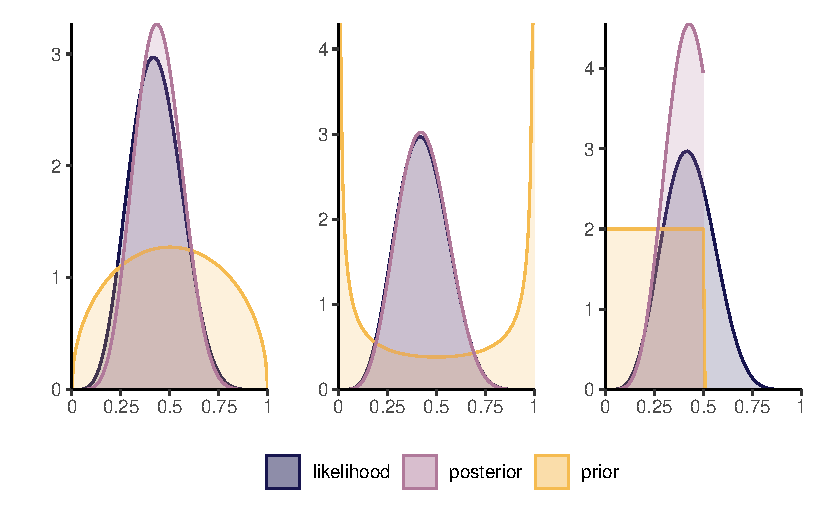
\includegraphics{introduction_files/figure-pdf/fig-betabinom-1.pdf}

}

\caption{\label{fig-betabinom}Scaled binomial likelihood for six
successes out of 14 trials, with \(\mathsf{Beta}(3/2, 3/2)\) prior
(left), \(\mathsf{Beta}(1/4, 1/4)\) (middle) and truncated uniform on
\([0,1/2]\) (right), with the corresponding posterior distributions.}

\end{figure}

\end{example}

\begin{remark}[Proportionality]

Any term appearing in the likelihood times prior function that does not
depend on parameters can be omitted since they will be absorbed by the
normalizing constant. This makes it useful to compute normalizing
constants or likelihood ratios.

\end{remark}

\begin{remark}

An alternative parametrization for the beta distribution sets
\(\alpha=\mu \kappa\), \(\beta = (1-\mu)\kappa\) for \(\mu \in (0,1)\)
and \(\kappa>0\), so that the model is parametrized directly in terms of
mean \(\mu\), with \(\kappa\) capturing the dispersion.

\end{remark}

\begin{remark}

A density integrates to 1 over the range of possible outcomes, but there
is no guarantee that the likelihood function, as a function of
\(\boldsymbol{\theta}\), integrates to one over the parameter domain
\(\boldsymbol{\Theta}\).

For example, the binomial likelihood with \(n\) trials and \(y\)
successes satisfies
\[\int_0^1 \binom{n}{y}\theta^y(1-\theta)^{n-y} \mathrm{d} \theta = \frac{1}{n+1}.\]

Moreover, the binomial distribution is discrete with support
\(0, \ldots, n\), whereas the likelihood is continuous as a function of
the probability of success, as evidenced by
Figure~\ref{fig-binom-massvslik}

\begin{figure}[ht!]

{\centering 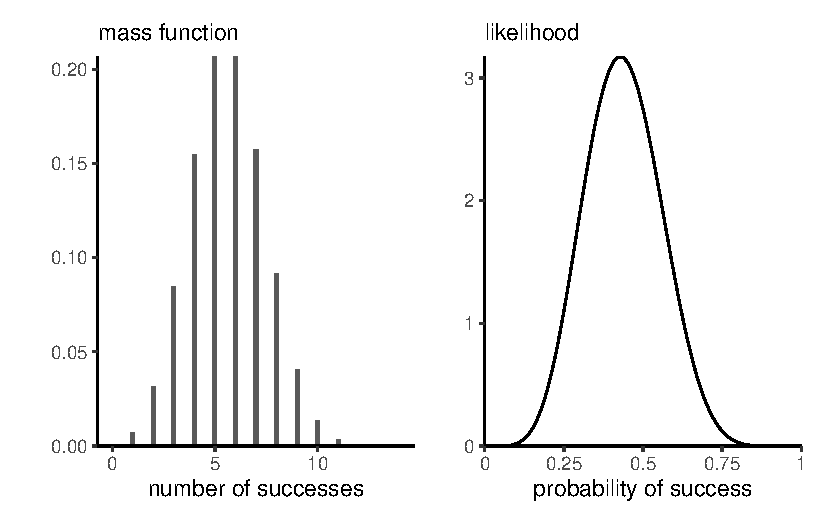
\includegraphics{introduction_files/figure-pdf/fig-binom-massvslik-1.pdf}

}

\caption{\label{fig-binom-massvslik}Binomial mass function (left) and
scaled likelihood function (right).}

\end{figure}

\end{remark}

\begin{proposition}[Sequentiality and Bayesian
updating]\protect\hypertarget{prp-sequentiality}{}\label{prp-sequentiality}

The likelihood is invariant to the order of the observations if they are
independent Thus, if we consider two blocks of observations
\(\boldsymbol{y}_1\) and \(\boldsymbol{y}_2\)
\[p(\boldsymbol{\theta} \mid \boldsymbol{y}_1, \boldsymbol{y}_2) = p(\boldsymbol{\theta} \mid \boldsymbol{y}_1) p(\boldsymbol{\theta} \mid \boldsymbol{y}_2),\]
so it makes no difference if we treat data all at once or in blocks.
More generally, for data exhibiting spatial or serial dependence, it
makes sense to consider rather the conditional (sequential)
decomposition
\[f(\boldsymbol{y}; \boldsymbol{\theta}) = f(\boldsymbol{y}_1; \boldsymbol{\theta}) f(\boldsymbol{y}_2; \boldsymbol{\theta}, \boldsymbol{y}_1) \cdots f(\boldsymbol{y}_n; \boldsymbol{\theta}, \boldsymbol{y}_1, \ldots, \boldsymbol{y}_{n-1})\]
where
\(f(\boldsymbol{y}_k; \boldsymbol{y}_1, \ldots, \boldsymbol{y}_{k-1})\)
denotes the conditional density function given observations
\(\boldsymbol{y}_1, \ldots, \boldsymbol{y}_{k-1}\).

By Bayes' rule, we can consider \emph{updating} the posterior by adding
terms to the likelihood, noting that \begin{align*}
p(\boldsymbol{\theta} \mid \boldsymbol{y}_1, \boldsymbol{y}_2) \propto p(\boldsymbol{y}_2 \mid \boldsymbol{y}_1, \boldsymbol{\theta}) p(\boldsymbol{\theta} \mid \boldsymbol{y}_1)
\end{align*} which amounts to treating the posterior
\(p(\boldsymbol{\theta} \mid \boldsymbol{y}_1)\) as a prior. If data are
exchangeable, the order in which observations are collected and the
order of the belief updating is irrelevant to the full posterior.
Figure~\ref{fig-sequential} shows how the posterior becomes gradually
closer to the scaled likelihood as we increase the sample size, and the
posterior mode moves towards the true value of the parameter (here 0.3).

\begin{figure}[ht!]

{\centering 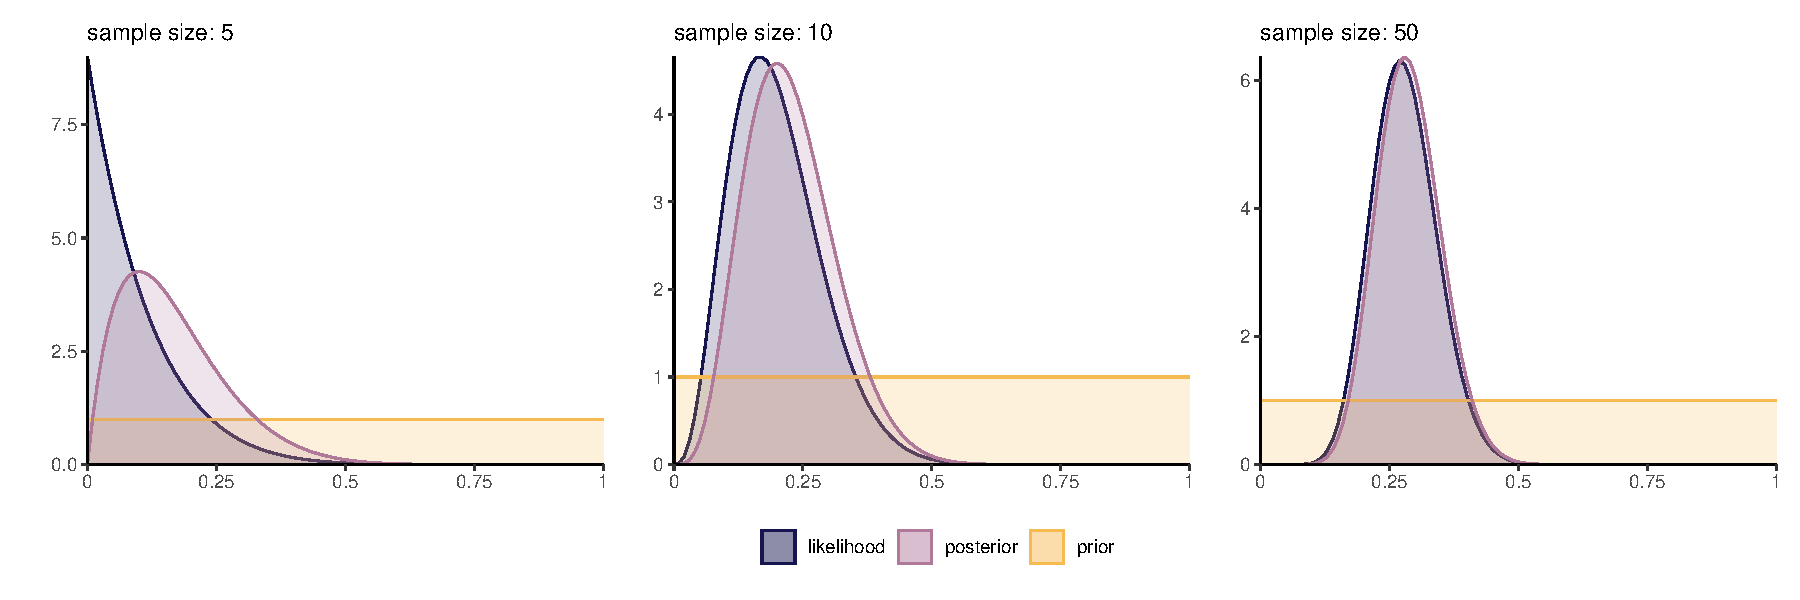
\includegraphics{introduction_files/figure-pdf/fig-sequential-1.pdf}

}

\caption{\label{fig-sequential}Beta posterior and binomial likelihood
with a uniform prior for increasing number of observations (from left to
right) out of a total of 100 trials.}

\end{figure}

\end{proposition}

\begin{example}[]\protect\hypertarget{exm-numericalintegration}{}\label{exm-numericalintegration}

While we can calculate analytically the value of the normalizing
constant for the beta-binomial model, we could also for arbitrary priors
use numerical integration or Monte Carlo methods in the event the
parameter vector \(\boldsymbol{\theta}\) is low-dimensional.

While estimation of the normalizing constant is possible in simple
models, the following highlights some challenges that are worth keeping
in mind. In a model for discrete data (that is, assigning probability
mass to a countable set of outcomes), the terms in the likelihood are
probabilities and thus the likelihood becomes smaller as we gather more
observations (since we multiply terms between zero or one). The marginal
likelihood term becomes smaller and smaller, so it's reciprocal is big
and this can lead to arithmetic underflow.

\begin{Shaded}
\begin{Highlighting}[]
\NormalTok{y }\OtherTok{\textless{}{-}}\NormalTok{ 6L }\CommentTok{\# number of successes }
\NormalTok{n }\OtherTok{\textless{}{-}}\NormalTok{ 14L }\CommentTok{\# number of trials}
\NormalTok{alpha }\OtherTok{\textless{}{-}}\NormalTok{ beta }\OtherTok{\textless{}{-}} \FloatTok{1.5} \CommentTok{\# prior parameters}
\NormalTok{unnormalized\_posterior }\OtherTok{\textless{}{-}} \ControlFlowTok{function}\NormalTok{(theta)\{}
\NormalTok{  theta}\SpecialCharTok{\^{}}\NormalTok{(y}\SpecialCharTok{+}\NormalTok{alpha}\DecValTok{{-}1}\NormalTok{) }\SpecialCharTok{*}\NormalTok{ (}\DecValTok{1}\SpecialCharTok{{-}}\NormalTok{theta)}\SpecialCharTok{\^{}}\NormalTok{(n}\SpecialCharTok{{-}}\NormalTok{y }\SpecialCharTok{+}\NormalTok{ beta }\SpecialCharTok{{-}} \DecValTok{1}\NormalTok{)}
\NormalTok{\}}
\FunctionTok{integrate}\NormalTok{(}\AttributeTok{f =}\NormalTok{ unnormalized\_posterior,}
          \AttributeTok{lower =} \DecValTok{0}\NormalTok{,}
          \AttributeTok{upper =} \DecValTok{1}\NormalTok{)}
\end{Highlighting}
\end{Shaded}

\begin{verbatim}
1.066906e-05 with absolute error < 1e-12
\end{verbatim}

\begin{Shaded}
\begin{Highlighting}[]
\CommentTok{\# Compare with known constant}
\FunctionTok{beta}\NormalTok{(y }\SpecialCharTok{+}\NormalTok{ alpha, n }\SpecialCharTok{{-}}\NormalTok{ y }\SpecialCharTok{+}\NormalTok{ beta)}
\end{Highlighting}
\end{Shaded}

\begin{verbatim}
[1] 1.066906e-05
\end{verbatim}

\begin{Shaded}
\begin{Highlighting}[]
\CommentTok{\# Monte Carlo integration}
\FunctionTok{mean}\NormalTok{(}\FunctionTok{unnormalized\_posterior}\NormalTok{(}\FunctionTok{runif}\NormalTok{(}\FloatTok{1e5}\NormalTok{)))}
\end{Highlighting}
\end{Shaded}

\begin{verbatim}
[1] 1.064067e-05
\end{verbatim}

\end{example}

When \(\boldsymbol{\theta}\) is high-dimensional, the marginal
likelihood is intractable. This is one of the main challenges of
Bayesian statistics and the popularity and applicability has grown
drastically with the development and popularity of numerical algorithms,
following th publication of Geman and Geman
(\protect\hyperlink{ref-Geman.Geman:1984}{1984}) and Gelfand and Smith
(\protect\hyperlink{ref-Gelfand.Smith:1990}{1990}). Markov chain Monte
Carlo methods circumvent the calculation of the denominator by drawing
approximate samples from the posterior.

\hypertarget{posterior-predictive-distribution}{%
\section{Posterior predictive
distribution}\label{posterior-predictive-distribution}}

Prediction in the Bayesian paradigm is obtained by considering the
\emph{posterior predictive distribution}, \begin{align*}
p(y_{\text{new}} \mid \boldsymbol{y}) =
\int_{\Theta} p(y_{\text{new}}  \mid \boldsymbol{\theta}) p(\boldsymbol{\theta} \mid  \boldsymbol{y}) \mathrm{d} \boldsymbol{\theta}
\end{align*}

Given draws from the posterior distribution, say
\(\boldsymbol{\theta}_b\) \((b=1, \ldots, B)\), we sample from each a
new realization from the distribution appearing in the likelihood
\(p(y_{\text{new}} \mid \boldsymbol{\theta}_b)\). This is different from
the frequentist setting, which fixes the value of the parameter to some
estimate \(\widehat{\boldsymbol{\theta}}\); by contrast, the posterior
predictive, here a beta-binomial distribution
\(\mathsf{BetaBin}(n, \alpha + y, n - y + \beta)\), carries over the
uncertainty so will typically be wider and overdispersed relative to the
corresponding binomial model. This can be easily seen from the
left-panel of Figure~\ref{fig-betabinompostpred}, which contrasts the
binomial mass function evaluated at the maximum likelihood estimator
\(\widehat{\theta}=6/14\) with the posterior predictive.

\begin{Shaded}
\begin{Highlighting}[]
\NormalTok{npost }\OtherTok{\textless{}{-}} \FloatTok{1e4}\NormalTok{L}
\CommentTok{\# Sample draws from the posterior distribution}
\NormalTok{post\_samp }\OtherTok{\textless{}{-}} \FunctionTok{rbeta}\NormalTok{(}\AttributeTok{n =}\NormalTok{ npost, y }\SpecialCharTok{+}\NormalTok{ alpha, n }\SpecialCharTok{{-}}\NormalTok{ y }\SpecialCharTok{+}\NormalTok{ beta)}
\CommentTok{\# For each draw, sample new observation}
\NormalTok{post\_pred }\OtherTok{\textless{}{-}} \FunctionTok{rbinom}\NormalTok{(}\AttributeTok{n =}\NormalTok{ npost, }\AttributeTok{size =}\NormalTok{ n, }\AttributeTok{prob =}\NormalTok{ post\_samp)}
\end{Highlighting}
\end{Shaded}

\begin{figure}[ht!]

{\centering 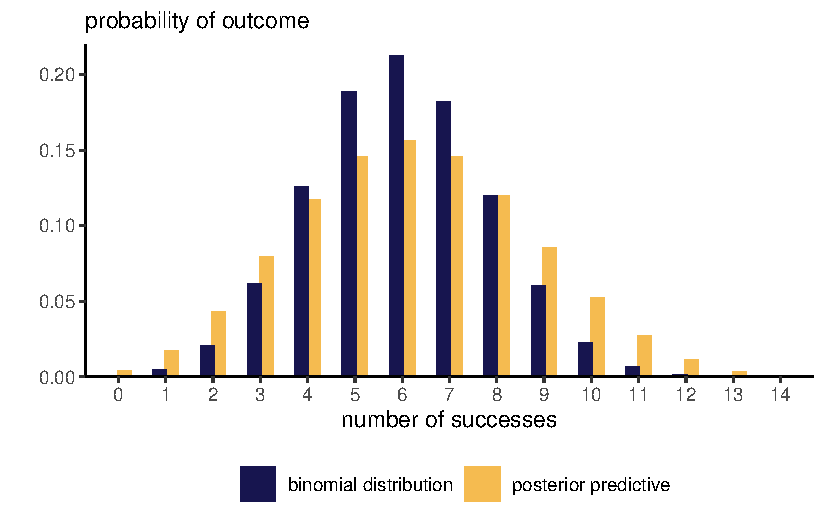
\includegraphics{introduction_files/figure-pdf/fig-betabinompostpred-1.pdf}

}

\caption{\label{fig-betabinompostpred}Beta-binomial posterior predictive
distribution with corresponding binomial mass function evaluated at the
maximum likelihood estimator.}

\end{figure}

\begin{example}[Posterior predictive distribution of univariate Gaussian
with known
mean]\protect\hypertarget{exm-normal-post-pred}{}\label{exm-normal-post-pred}

Consider an \(n\) sample of independent and identically distributed
Gaussian, \(Y_i \sim \mathsf{No}(0, \tau^{-1})\) (\(i=1, \ldots, n\)),
where we assign a gamma prior on the precision
\(\tau \sim \mathsf{Ga}(\alpha, \beta)\). The posterior is
\begin{align*}
p(\tau \mid \boldsymbol{y}) \stackrel{\tau}{\propto} \prod_{i=1}^n \tau^{n/2}\exp\left(-\tau \frac{\sum_{i=1}^n{y_i^2}}{2}\right) \times \tau^{\alpha-1} \exp(-\beta \tau)
\end{align*} and rearranging the terms to collect powers of \(\tau\),
etc. we find that the posterior for \(\tau\) must also be gamma, with
shape parameter \(\alpha^* = \alpha + n/2\) and rate
\(\beta^* = \beta + \sum_{i=1}^n y_i^2/2\).

The posterior predictive is \begin{align*}
p(y_{\text{new}} \mid \boldsymbol{y}) &= \int_0^\infty \frac{\tau^{1/2}}{(2\pi)^{1/2}}\exp(-\tau y_{\text{new}}^2/2) \frac{\beta^{*\alpha^*}}{\Gamma(\alpha^*)}\tau^{\alpha^*-1}\exp(-\beta^* \tau) \mathrm{d} \tau 
\\&= (2\pi)^{-1/2} \frac{\beta^{*\alpha^*}}{\Gamma(\alpha^*)} \int_0^\infty\tau^{\alpha^*-1/2} \exp\left\{- \tau (y_{\text{new}}^2/2 + \beta^*)\right\} \mathrm{d} \tau
\\&= (2\pi)^{-1/2} \frac{\beta^{*\alpha^*}}{\Gamma(\alpha^*)} \frac{\Gamma(\alpha^* + 1/2)}{(y_{\text{new}}^2/2 + \beta^*)^{\alpha^*+1/2}}
\\&= \frac{\Gamma\left(\frac{2\alpha^* + 1}{2}\right)}{\sqrt{2\pi}\Gamma\left(\frac{2\alpha^*}{2}\right)\beta^{*1/2}} \left( 1+ \frac{y_{\text{new}}^2}{2\beta^*}\right)^{-\alpha^*-1/2}
\\&= \frac{\Gamma\left(\frac{2\alpha^* + 1}{2}\right)}{\sqrt{\pi}\sqrt{ 2\alpha^*}\Gamma\left(\frac{2\alpha^*}{2}\right)(\beta^*/\alpha^*)^{1/2}} \left( 1+ \frac{1}{2\alpha^*}\frac{y_{\text{new}}^2}{(\beta^*/\alpha^*)}\right)^{-\alpha^*-1/2}
\end{align*} which entails that \(Y_{\text{new}}\) is a scaled
Student-\(t\) distribution with scale \((\beta^*/\alpha^*)^{1/2}\) and
\(2\alpha+n\) degrees of freedom. This example also exemplifies the
additional variability relative to the distribution generating the data:
indeed, the Student-\(t\) distribution is more heavy-tailed than the
Gaussian, but since the degrees of freedom increase linearly with \(n\),
the distribution converges to a Gaussian as \(n \to \infty\), reflecting
the added information as we collect more and more data points and the
variance gets better estimated through \(\sum_{i=1}^n y_i^2/n\).

\end{example}

\hypertarget{summarizing-posterior-distributions}{%
\section{Summarizing posterior
distributions}\label{summarizing-posterior-distributions}}

The output of the Bayesian learning problem will be either of:

\begin{enumerate}
\def\labelenumi{\arabic{enumi}.}
\tightlist
\item
  a fully characterized distribution
\item
  a numerical approximation to the posterior distribution (pointwise)
\item
  an exact or approximate sample drawn from the posterior distribution
\end{enumerate}

In the first case, we will be able to directly evaluate quantities of
interest if there are closed-form expressions for the latter, or else we
could draw samples from the distribution and evaluate them via
Monte-Carlo. In case of numerical approximations, we will need to resort
to numerical integration or otherwise to get our answers.

Often, we will also be interested in the marginal posterior distribution
of each component \(\theta_j\) in turn (\(j=1, \ldots, J\)). To get
these, we carry out additional integration steps,
\[p(\theta_j \mid \boldsymbol{y}) = \int p(\boldsymbol{\theta} \mid \boldsymbol{y}) \mathrm{d} \boldsymbol{\theta}_{-j}.\]
With a posterior sample, this is trivial: it suffices to keep the column
corresponding to \(\theta_j\) and discard the others.

Most of the field of Bayesian statistics revolves around the creation of
algorithms that either circumvent the calculation of the normalizing
constant (notably using Monte Carlo and Markov chain Monte Carlo
methods) or else provide accurate numerical approximation of the
posterior pointwise, including for marginalizing out all but one
parameters (integrated nested Laplace approximations, variational
inference, etc.) The target of inference is the whole posterior
distribution, a potentially high-dimensional object which may be
difficult to summarize or visualize. We can thus report only
characteristics of the the latter.

The choice of point summary to keep has it's root in decision theory.

\begin{definition}[Loss
function]\protect\hypertarget{def-lossfunction}{}\label{def-lossfunction}

A loss function \(c(\boldsymbol{\theta}, \boldsymbol{\upsilon})\) is a
mapping from \(\boldsymbol{\Theta} \to \mathbb{R}^k\) that assigns a
weight to each value of \(\boldsymbol{\theta}\), corresponding to the
regret or loss arising from choosing this value. The corresponding point
estimator \(\widehat{\boldsymbol{\upsilon}}\) is the minimizer of the
expected loss,

\[\widehat{\boldsymbol{\upsilon}} = \mathop{\mathrm{argmin}}_{\boldsymbol{\upsilon}} \int_{\boldsymbol{\Theta}} c(\boldsymbol{\theta}, \boldsymbol{\upsilon})p(\boldsymbol{\theta} \mid \boldsymbol{y}) \mathrm{d} \boldsymbol{\theta}\]

\end{definition}

For example, in a univariate setting, the quadratic loss
\(c(\theta, \upsilon) = (\theta-\upsilon)^2\) returns the posterior
mean, the absolute loss \(c(\theta, \upsilon)=|\theta - \upsilon|\)
returns the posterior median and the 0-1 loss
\(c(\theta, \upsilon) = \mathrm{I}(\upsilon \neq \theta)\) returns the
posterior mode. All of these point estimators are central tendency
measures, but some may be more adequate depending on the setting as they
can correspond to potentially different values, as shown in the
left-panel of Figure~\ref{fig-central-moments}. The choice is
application specific: for multimodal distributions, the mode is likely a
better choice.

If we know how to evaluate the distribution numerically, we can optimize
to find the mode or else return the value for the pointwise evaluation
on a grid at which the density achieves it's maximum. The mean and
median would have to be evaluated by numerical integration if there is
no closed-form expression for the latter.

If we have rather a sample from the posterior with associated posterior
density values, then we can obtain the mode as the parameter combination
with the highest posterior, the median from the value at rank
\(\lfloor n/2\rfloor\) and the mean through the sample mean of posterior
draws.

\begin{figure}[ht!]

{\centering 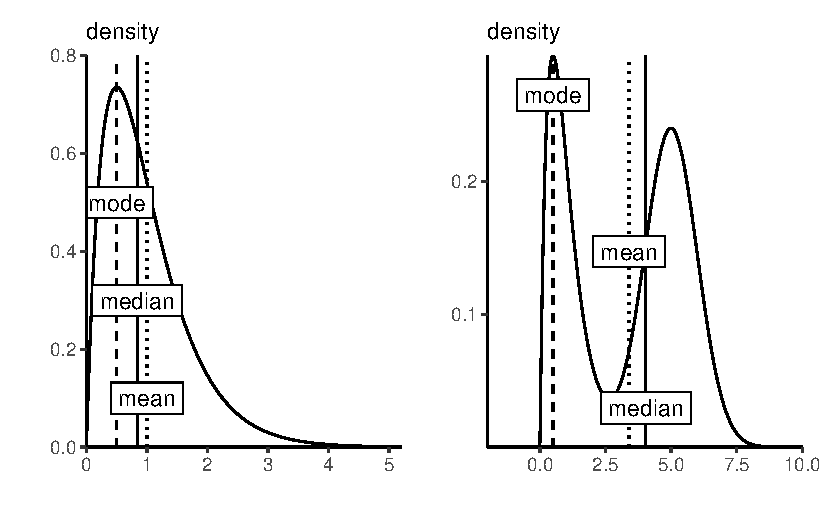
\includegraphics{introduction_files/figure-pdf/fig-central-moments-1.pdf}

}

\caption{\label{fig-central-moments}Point estimators from a right-skewed
distribution (left) and from a multimodal distribution (right).}

\end{figure}

The loss function is often a functional (meaning a one-dimensional
summary) from the posterior. The following example shows how it reduces
a three-dimensional problem into a single risk measure.

\begin{example}[Danish insurance
losses]\protect\hypertarget{exm-loss-extremes}{}\label{exm-loss-extremes}

In extreme value, we are often interested in assessing the risk of
events that are rare enough that they lie beyond the range of observed
data. To provide a scientific extrapolation, it often is justified to
fit a generalized Pareto distribution to exceedances of \(Z=Y-u\), for
some user-specified threshold \(u\) which is often taken as a large
quantile of the distribution of \(Y\). The generalized Pareto
distribution function is \begin{align*}
F(z; \tau, \xi) = 1- \begin{cases}
\left(1+\xi/\tau z\right)^{-1/\xi}_{+}, & \xi \neq 0\\
\exp(-z/\tau), & \xi = 0. \end{cases}
\end{align*} The shape \(\xi\) governs how heavy-tailed the distribution
is, while \(\tau\) is a scale parameter.

Insurance companies provide coverage in exchange for premiums, but need
to safeguard themselves against very high claims by buying reinsurance
products. These risks are often communicated through the value-at-risk
(VaR), a high quantile exceeded with probability \(p\). We model Danish
fire insurance claim amounts for inflation-adjusted data collected from
January 1980 until December 1990 that are in excess of a million Danish
kroner, found in the \texttt{evir} package and analyzed in Example 7.23
of McNeil, Frey, and Embrechts
(\protect\hyperlink{ref-McNeil.Frey.Embrechts:2005}{2005}). These claims
are denoted \(Y\) and there are 2167 observations.

We fit a generalized Pareto distribution to exceedances above 10
millions krones, keeping 109 observations or roughly the largest 5\% of
the original sample. Preliminary analysis shows that we can treat data
as roughly independent and identically distributed and goodness-of-fit
diagnostics (not shown) for the generalized Pareto suggest that the fit
is adequate for all but the three largest observations, which are
(somewhat severely) underestimated by the model.

\begin{figure}[ht!]

{\centering 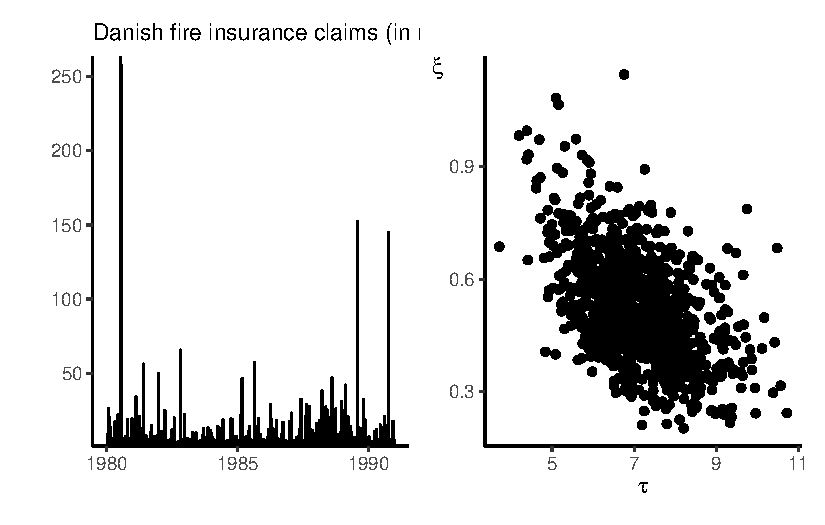
\includegraphics{introduction_files/figure-pdf/fig-danish-1.pdf}

}

\caption{\label{fig-danish}Time series of Danish fire claims exceeding a
million krone (left) and posterior samples from the scale \(\tau\) and
shape \(\xi\) of the generalized Pareto model fitted to exceedances
above 10 million krone (right).}

\end{figure}

The generalized Pareto model only describes the \(n_u\) exceedances
above \(u=10\), so we need to incorporate in the likelihood a binomial
contribution for the probability \(\zeta_u\) of exceeding the threshold
\(u\). Provided that the priors for \((\tau, \xi)\) are independent of
those for \(\zeta_u\), the posterior also factorizes as a product, so
\(\zeta_u\) and \((\tau, \xi)\) are a posteriori independent.

Suppose for now that we set a \(\mathsf{Be}(0.5, 0.5)\) prior for
\(\zeta_u\) and a non-informative prior for the generalized Pareto
parameters. The \texttt{post\_samp} matrix contains exact samples from
the posterior distribution of \((\tau, \xi, \zeta_u)\), obtained using a
Monte Carlo algorithm. Our aim is to evaluate the posterior distribution
for the value-at-risk, the \(\alpha\) quantile of \(Y\) for high values
of \(\alpha\) and see what point estimator one would obtain depending on
our choice of loss function. For any \(\alpha > 1-\zeta_u\), the
\(q_{\alpha}\) is \begin{align*}
1- \alpha  &= \Pr(Y > q_\alpha \mid Y > u) \Pr(Y > u) 
\\ &= \left(1+\xi \frac{q_{\alpha}-u}{\tau}\right)_{+}^{-1/\xi}\zeta_u
\end{align*} and solving for \(q_{\alpha}\) gives \begin{align*}
q_{\alpha} = u+ \frac{\tau}{\xi} \left\{\left(\frac{\zeta_u}{1-\alpha}\right)^\xi-1\right\}.
\end{align*}

To obtain the posterior distribution of the \(\alpha\) quantile,
\(q_{\alpha}\), it suffices to plug in each posterior sample and
evaluate the function: the uncertainty is carried over from the
simulated values of the parameters to those of the quantile
\(q_{\alpha}\). The left panel of Figure~\ref{fig-lossfn} shows the
posterior density estimate of the \(\mathsf{VaR}(0.99)\) along with the
maximum a posteriori (mode) of the latter.

Suppose that we prefer to under-estimate the value-at-risk rather than
overestimate: this could be captured by the custom loss function
\begin{align*}
c(q, q_0) = 
\begin{cases}
0.5(0.99q - q_0), & q > q_0 \\
0.75(q_0 - 1.01q), & q < q_0.
\end{cases}
\end{align*} For a given value of the value-at-risk \(q_0\) evaluated on
a grid, we thus compute \begin{align*}
 r(q_0) = \int_{\boldsymbol{\Theta}}c(q(\boldsymbol{\theta}), q_0) p (\boldsymbol{\theta} \mid \boldsymbol{y}) \mathrm{d} \boldsymbol{\theta}
\end{align*} and we seek to minimize the risk,
\(\widehat{q} =\mathrm{argmin}_{q_0 \in \mathbb{R}_{+}} r(q_0)\). The
value returned that minimizes the loss, shown in
Figure~\ref{fig-lossfn}, is to the left of the posterior mean for
\(q_\alpha\).

\begin{Shaded}
\begin{Highlighting}[]
\CommentTok{\# Compute value at risk from generalized Pareto distribution quantile fn}
\NormalTok{VaR\_post }\OtherTok{\textless{}{-}} \FunctionTok{with}\NormalTok{(post\_samp,   }\CommentTok{\# data frame of posterior draws}
\NormalTok{            revdbayes}\SpecialCharTok{::}\FunctionTok{qgp}\NormalTok{(   }\CommentTok{\# with columns \textquotesingle{}probexc\textquotesingle{}, \textquotesingle{}scale\textquotesingle{}, \textquotesingle{}shape\textquotesingle{}}
  \AttributeTok{p =} \FloatTok{0.01}\SpecialCharTok{/}\NormalTok{probexc, }
  \AttributeTok{loc =} \DecValTok{10}\NormalTok{, }
  \AttributeTok{scale =}\NormalTok{ scale, }
  \AttributeTok{shape =}\NormalTok{ shape, }
  \AttributeTok{lower.tail =} \ConstantTok{FALSE}\NormalTok{))}
\CommentTok{\# Loss function}
\NormalTok{loss }\OtherTok{\textless{}{-}} \ControlFlowTok{function}\NormalTok{(qhat, q)\{}
    \FunctionTok{mean}\NormalTok{(}\FunctionTok{ifelse}\NormalTok{(q }\SpecialCharTok{\textgreater{}}\NormalTok{ qhat,}
           \FloatTok{0.5}\SpecialCharTok{*}\NormalTok{(}\FloatTok{0.99}\SpecialCharTok{*}\NormalTok{q}\SpecialCharTok{{-}}\NormalTok{qhat),}
           \FloatTok{0.75}\SpecialCharTok{*}\NormalTok{(qhat}\FloatTok{{-}1.01}\SpecialCharTok{*}\NormalTok{q)))}
\NormalTok{\}}
\CommentTok{\# Create a grid of values over which to estimate the loss for VaR}
\NormalTok{nvals }\OtherTok{\textless{}{-}}\NormalTok{ 101L}
\NormalTok{VaR\_grid }\OtherTok{\textless{}{-}} \FunctionTok{seq}\NormalTok{(}
  \AttributeTok{from =} \FunctionTok{quantile}\NormalTok{(VaR\_post, }\FloatTok{0.01}\NormalTok{),}
  \AttributeTok{to =} \FunctionTok{quantile}\NormalTok{(VaR\_post, }\FloatTok{0.99}\NormalTok{), }
  \AttributeTok{length.out =}\NormalTok{ nvals)}
\CommentTok{\# Create a container to store results}
\NormalTok{risk }\OtherTok{\textless{}{-}} \FunctionTok{numeric}\NormalTok{(}\AttributeTok{length =}\NormalTok{ nvals)}
\ControlFlowTok{for}\NormalTok{(i }\ControlFlowTok{in} \FunctionTok{seq\_len}\NormalTok{(nvals))\{}
  \CommentTok{\# Compute integral (Monte Carlo average over draws)}
\NormalTok{ risk[i] }\OtherTok{\textless{}{-}} \FunctionTok{loss}\NormalTok{(}\AttributeTok{q =}\NormalTok{ VaR\_post, }\AttributeTok{qhat =}\NormalTok{ VaR\_grid[i])}
\NormalTok{\}}
\end{Highlighting}
\end{Shaded}

\begin{figure}[ht!]

{\centering 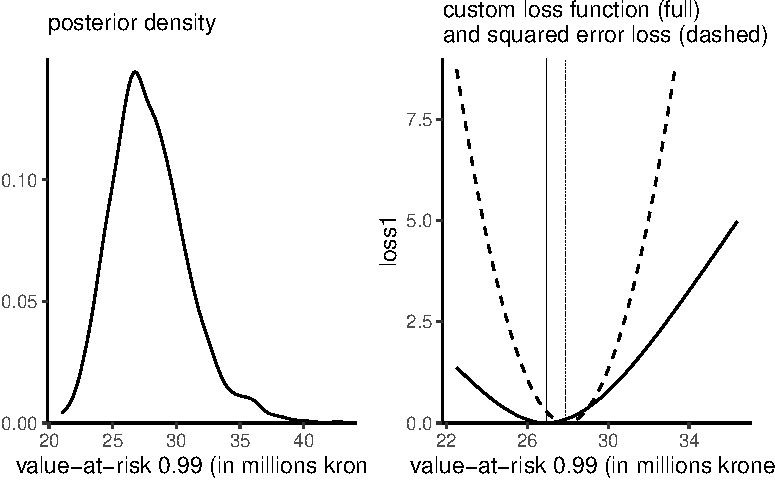
\includegraphics{introduction_files/figure-pdf/fig-lossfn-1.pdf}

}

\caption{\label{fig-lossfn}Posterior density (left) and losses functions
for the 0.99 value-at-risk for the Danish fire insurance data. The
vertical lines denote point estimates of the quantiles that minimize the
loss functions.}

\end{figure}

\end{example}

To communicate uncertainty, we may resort to credible regions and
intervals.

\begin{definition}[]\protect\hypertarget{def-credible-region}{}\label{def-credible-region}

A \((1-\alpha)\) \textbf{credible region} (or credible interval in the
univariate setting) is a set \(\mathcal{S}_\alpha\) such that, with
probability level \(\alpha\), \begin{align*}
\Pr(\boldsymbol{\theta} \in \mathcal{S}_\alpha \mid \boldsymbol{Y}=\boldsymbol{y}) = 1-\alpha
\end{align*}

\end{definition}

These intervals are not unique, as are confidence sets. In the
univariate setting, the central or equitailed interval are the most
popular, and easily obtained by considering the \(\alpha/2, 1-\alpha/2\)
quantiles. These are easily obtained from samples by simply taking
empirical quantiles. An alternative, highest posterior density credible
sets, which may be a set of disjoint intervals obtained by considering
the parts of the posterior with the highest density, may be more
informative. The top panel Figure~\ref{fig-credible-intervals} shows the
distinction for a bimodal mixture distribution, and a even more striking
difference for 50\% credible intervals for a symmetric beta distribution
whose mass lie near the endpoints of the distribution, leading to no
overlap between the two intervals.

\begin{figure}[ht!]

{\centering 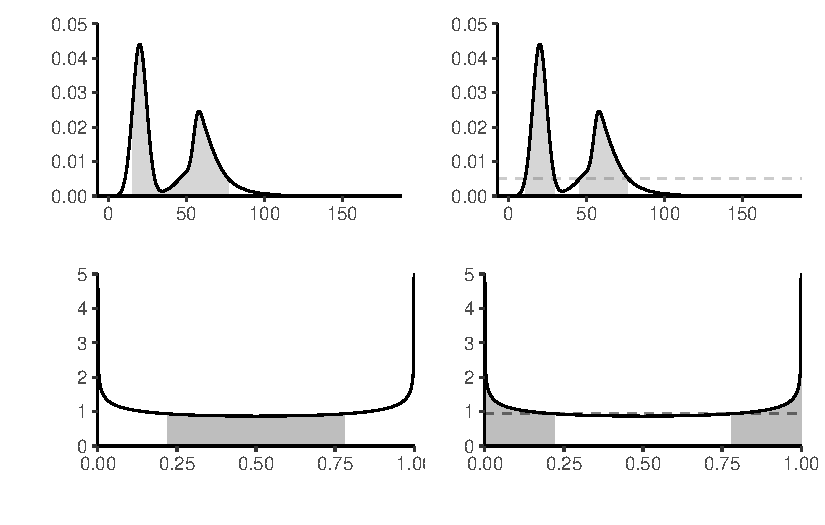
\includegraphics{introduction_files/figure-pdf/fig-credible-intervals-1.pdf}

}

\caption{\label{fig-credible-intervals}Density plots with 89\% (top) and
50\% (bottom) equitailed or central credible (left) and highest
posterior density (right) regions for two data sets, highlighted in
grey.}

\end{figure}

\bookmarksetup{startatroot}

\hypertarget{priors}{%
\chapter{Priors}\label{priors}}

The posterior distribution combines two ingredients: the likelihood and
the prior. If the former is a standard ingredient of any
likelihood-based inference, prior specification requires some care. The
purpose of this chapter is to consider different standard way of
constructing prior functions, and to specify the parameters of the
latter: we term these hyperparameters.

\hypertarget{conjugate-priors}{%
\section{Conjugate priors}\label{conjugate-priors}}

In very simple models, there may exists prior densities that result in a
posterior distribution of the same family. We can thus directly extract
characteristics of the posterior. Conjugate priors are chosen for
computational convenience and because interpretation is convenient, as
the parameters of the posterior will often be some weighted average of
prior and likelihood component.

\begin{definition}[]\protect\hypertarget{def-conjugate-prior}{}\label{def-conjugate-prior}

A prior density \(p(\boldsymbol{\theta})\) is conjugate for likelihood
\(L(\boldsymbol{\theta}; \boldsymbol{y})\) if the product
\(L(\boldsymbol{\theta}; \boldsymbol{y})p(\boldsymbol{\theta})\), after
renormalization, is of the same parametric family as the prior.

Exponential families (including the binomial, Poisson, exponential,
Gaussian distributions) admit conjugate priors\footnote{A distribution
  belongs to an exponential family with parameter vector
  \(\boldsymbol{\theta} \in \mathbb{R}^D\) if it can be written as
  \begin{align*}
  f(y; \boldsymbol{\theta}) = \exp\left\{ \sum_{k=1}^K Q_k(\boldsymbol{\theta}) t_k(y) + D(\boldsymbol{\theta})\right\}
  \end{align*} and in particular, the support does not depend on unknown
  parameters. If we have an independent and identically distributed
  sample of observations \(y_1, \ldots, y_n\), the log likelihood is
  thus of the form \begin{align*}
  \ell(\boldsymbol{\theta}) = \sum_{k=1}^K \phi_k(\boldsymbol{\theta}) \sum_{i=1}^n t_k(y_i) + n D(\boldsymbol{\theta}),
  \end{align*} where the collection \(\sum_{i=1}^n t_k(y_i)\)
  (\(k=1, \ldots, K\)) are sufficient statistics and
  \(\phi_k(\boldsymbol{\theta})\) are the canonical parameters. The
  number of sufficient statistics are the same regardless of the sample
  size. Exponential families play a prominent role in generalized linear
  models, in which the natural parameters are modeled as linear function
  of explanatory variables. A log prior density with parameters
  \(\eta, \nu_1, \ldots, \nu_K\) that is proportional to \begin{align*}
  \log p(\boldsymbol{\theta}) \propto \eta D(\boldsymbol{\theta}) + \sum_{k=1}^K Q_k(\boldsymbol{\theta}) \nu_k
  \end{align*} is conjugate.}

\end{definition}

\begin{example}[Conjugate prior for the binomial
model]\protect\hypertarget{exm-conjugatepriors-binom}{}\label{exm-conjugatepriors-binom}

The binomial log density with \(y\) successes out of \(n\) trials is
proportional to \begin{align*}
y \log(p) + (n-y) \log(1-p) = y\log\left( \frac{p}{1-p}\right) + n \log(1-p)
\end{align*} with canonical parameter \(\mathrm{logit}(p)\).\footnote{The
  canonical link function for Bernoulli gives rise to logistic
  regression model.} The binomial distribution is thus an exponential
family.

Since the density of the binomial is of the form \(p^y(1-p)^{n-y}\), the
beta distribution \(\mathsf{Be}(\alpha, \beta)\) with density
\[f(x) \propto x^{\alpha-1} (1-x)^{\beta-1}\] is the conjugate prior.

The beta distribution is also the conjugate prior for the negative
binomial, geometric and Bernoulli distributions, since their likelihoods
are all proportional to that of the beta. The fact that different
sampling schemes that result in proportional likelihood functions give
the same inference is called likelihood principle.

\end{example}

\begin{example}[Conjugate prior for the Poisson
model]\protect\hypertarget{exm-conjugatepriors-poisson}{}\label{exm-conjugatepriors-poisson}

The Poisson distribution with mean \(\mu\) has log density proportional
to \(f(y; \mu) \propto y\log(\mu) -\mu\), so is an exponential family
with natural parameter \(\log(\mu)\). The gamma density,
\[ f(x) \propto \beta^{\alpha}/\Gamma(\alpha)x^{\alpha-1} \exp(-\beta x)\]
with shape \(\alpha\) and rate \(\beta\) is the conjugate prior for the
Poisson. For an \(n\)-sample of independent observations
\(\mathsf{Po}(\mu)\) observations with
\(\mu \sim \mathsf{Ga}(\alpha, \beta)\), the posterior is
\(\mathsf{Ga}(\sum_{i=1}^n y_i + \alpha, \beta + n)\).

\end{example}

Knowing the analytic expression for the posterior can be useful for
calculations of the marginal likelihood, as
Example~\ref{exm-poisson-negbin} demonstrates.

\begin{example}[Negative binomial as a Poisson
mixture]\protect\hypertarget{exm-poisson-negbin}{}\label{exm-poisson-negbin}

~

One restriction of the Poisson model is that the restriction on its
moments is often unrealistic. The most frequent problem encountered is
that of \textbf{overdispersion}, meaning that the variability in the
counts is larger than that implied by a Poisson distribution.

One common framework for handling overdispersion is to have
\(Y \mid \Lambda = \lambda \sim \mathsf{Po}(\lambda)\), where the mean
of the Poisson distribution is itself a positive random variable with
mean \(\mu\), if \(\Lambda\) follows a conjugate gamma distribution with
shape \(k\mu\) and rate \(k>0\), \(\Lambda \sim \mathsf{Ga}(k\mu, k)\),
the posterior \(\Lambda \mid Y=y \sim \mathsf{Ga}(k\mu + y, k+1)\).

Since the joint density of \(Y\) and \(\Lambda\) can be written \[
p(y, \lambda) = p(y \mid \lambda)p(\lambda) = p(\lambda \mid y) p(y)
\] we can isolate the marginal density \begin{align*}
p(y) &= \frac{p(y \mid \lambda)p(\lambda)}{p(\lambda \mid y)} \\&= \frac{\frac{\lambda^y\exp(-\lambda)}{\Gamma(y+1)}  \frac{k^{k\mu}\lambda^{k\mu-1}\exp(-k\lambda)}{\Gamma(k\mu)}}{ \frac{(k+1)^{k\mu+y}\lambda^{k\mu+y-1}\exp\{-(k+1)\lambda\}}{\Gamma(k\mu+y)}}\\
&= \frac{\Gamma(k\mu+y)}{\Gamma(k\mu)\Gamma(y+1)}k^{k\mu} (k+1)^{-k\mu-y}\\&= \frac{\Gamma(k\mu+y)}{\Gamma(k\mu)\Gamma(y+1)}\left(1-\frac{1}{k+1}\right)^{k\mu} \left(\frac{1}{k+1}\right)^y
\end{align*} and this is the density of a negative binomial distribution
with probability of success \(1/(k+1)\). We can thus view the negative
binomial as a Poisson mean mixture.

By the laws of iterated expectation and iterative variance,
\begin{align*}
\mathsf{E}(Y) &= \mathsf{E}_{\Lambda}\{\mathsf{E}(Y \mid \Lambda\} \\& = \mathsf{E}(\Lambda) = \mu\\
\mathsf{Va}(Y) &= \mathsf{E}_{\Lambda}\{\mathsf{Va}(Y \mid \Lambda)\} + \mathsf{Va}_{\Lambda}\{\mathsf{E}(Y \mid \Lambda)\} \\&= \mathsf{E}(\Lambda) + \mathsf{Va}(\Lambda) \\&= \mu + \mu/k.
\end{align*} The marginal distribution of \(Y\), unconditionally, has a
variance which exceeds its mean, as \begin{align*}
\mathsf{E}(Y) = \mu, \qquad \mathsf{Va}(Y) = \mu (1+1/k).
\end{align*} In a negative binomial regression model, the term \(k\) is
a dispersion parameter, which is fixed for all observations, whereas
\(\mu = \exp(\boldsymbol{\beta}\mathbf{X})\) is a function of covariates
\(\mathbf{X}\). As \(k \to \infty\), the distribution of \(\Lambda\)
degenerates to a constant at \(\mu\) and we recover the Poisson model.

\end{example}

\begin{example}[Posterior rates for A/B tests using conjugate Poisson
model]\protect\hypertarget{exm-abtest}{}\label{exm-abtest}

Upworthy.com, a US media publisher, revolutionized headlines online
advertisement by running systematic A/B tests to compare the different
wording of headlines, placement and image and what catches attention the
most. The Upworthy Research Archive
(\protect\hyperlink{ref-Matias:2021}{Matias et al. 2021}) contains
results for 22743 experiments, with a click through rate of 1.58\% on
average and a standard deviation of 1.23\%. The
\texttt{clickability\_test\_id} gives the unique identifier of the
experiment, \texttt{clicks} the number of conversion out of
\texttt{impressions}. See
\href{https://tellingstorieswithdata.com/08-hunt.html\#ab-testing}{Section
8.5} of Alexander (\protect\hyperlink{ref-Alexander:2023}{2023}) for
more details about A/B testing and background information.

Consider an A/B test from November 23st, 2014, that compared four
different headlines for a story on Sesame Street workshop with
interviews of children whose parents were in jail and visiting them in
prisons. The headlines tested were:

\begin{quote}
\begin{enumerate}
\def\labelenumi{\arabic{enumi}.}
\tightlist
\item
  Some Don't Like It When He Sees His Mom. But To Him? Pure Joy. Why
  Keep Her From Him?
\item
  They're Not In Danger. They're Right. See True Compassion From The
  Children Of The Incarcerated.
\item
  Kids Have No Place In Jail \ldots{} But In This Case, They
  \emph{Totally} Deserve It.
\item
  Going To Jail \emph{Should} Be The Worst Part Of Their Life. It's So
  Not. Not At All.
\end{enumerate}
\end{quote}

At first glance, the first and third headlines seem likely to lead to a
curiosity gap. The wording of the second is more explicit (and
searchable), whereas the first is worded as a question.

We model the conversion rate \(\lambda_i\) for each headline separately
using a Poisson distribution and compare the posterior distributions for
all four choices. Using a conjugate prior and selecting the parameters
by moment matching yields approximately \(\alpha = 1.64\) and
\(\beta = 0.01\) for the hyperparameters.

\hypertarget{tbl-upworthy}{}
\begin{longtable}[]{@{}lrr@{}}
\caption{\label{tbl-upworthy}Number of views, clicks for different
headlines for the Upworthy data.}\tabularnewline
\toprule\noalign{}
headline & impressions & clicks \\
\midrule\noalign{}
\endfirsthead
\toprule\noalign{}
headline & impressions & clicks \\
\midrule\noalign{}
\endhead
\bottomrule\noalign{}
\endlastfoot
H1 & 3060 & 49 \\
H2 & 2982 & 20 \\
H3 & 3112 & 31 \\
H4 & 3083 & 9 \\
\end{longtable}

\begin{figure}[ht!]

{\centering 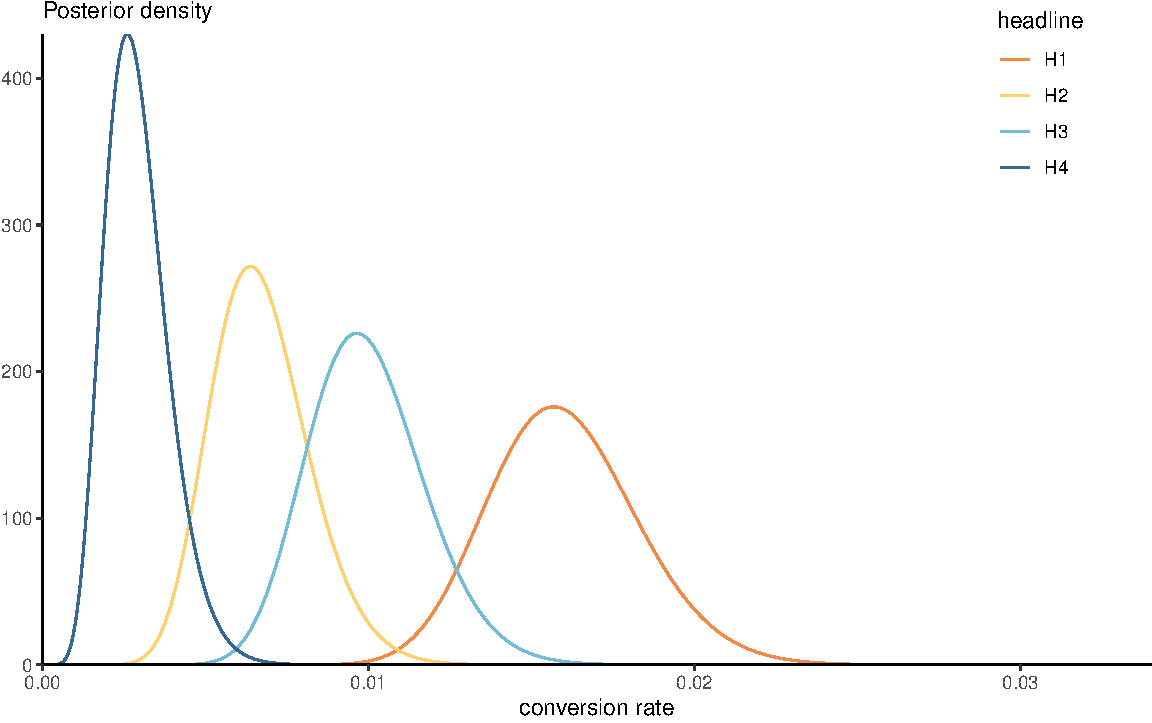
\includegraphics{priors_files/figure-pdf/fig-upworthy-1.pdf}

}

\caption{\label{fig-upworthy}Gamma posterior for the Upworthy Sesame
street headline.}

\end{figure}

We can visualize the posterior distributions. In this context, the large
sample size lead to the dominance of the likelihood contribution
\(p(Y_i \mid \lambda_i) \sim \mathsf{Po}(n_i\lambda_i)\) relative to the
prior. We can see there is virtually no overlap between different rates
for headers H1 (preferred) relative to H4 (least favorable). The
probability that the conversion rate for Headline 3 is higher than
Headline 1 can be approximated by simulating samples from both
posteriors and computing the proportion of times one is larger: we get
1.7\% for \texttt{H3} relative to \texttt{H1}, indicating a clear
preference for the first headline \texttt{H1}.

\end{example}

\begin{example}[Should you phrase your headline as a
question?]\protect\hypertarget{exm-poisson-upworthy-question}{}\label{exm-poisson-upworthy-question}

We can also consider aggregate records for Upworthy, as Alexander
(\protect\hyperlink{ref-Alexander:2023}{2023}) did. The
\texttt{upworthy\_question} database contains a balanced sample of all
headlines where at least one of the choices featured a question, with at
least one alternative statement. Whether a headline contains a question
or not is determined by querying for the question mark. We consider
aggregated counts for all such headlines, with the \texttt{question}
factor encoding whether there was a question, \texttt{yes} or
\texttt{no}. For simplicity, we treat the number of views as fixed, but
keep in mind that A/B tests are often sequential experiments with a
stopping rule.\footnote{The stopping rule means that data stops being
  collected once there is enough evidence to determine if an option is
  more suitable, or if a predetermined number of views has been reached.}

We model first the rates using a Poisson regression; the corresponding
frequentist analysis would include an offset to account for differences
in views. If \(\lambda_{j}\) \((j=1, 2)\) are the average rate for each
factor level (yes and no), then
\(\mathsf{E}(Y_{ij}/n_{ij}) = \lambda_j\). In the frequentist setting,
we can fit a simple Poisson generalized linear regression model with an
offset term and a binary variable.

\begin{Shaded}
\begin{Highlighting}[]
\FunctionTok{data}\NormalTok{(upworthy\_question, }\AttributeTok{package =} \StringTok{"hecbayes"}\NormalTok{)}
\NormalTok{poismod }\OtherTok{\textless{}{-}} \FunctionTok{glm}\NormalTok{(}
\NormalTok{  clicks }\SpecialCharTok{\textasciitilde{}} \FunctionTok{offset}\NormalTok{(}\FunctionTok{log}\NormalTok{(impressions)) }\SpecialCharTok{+}\NormalTok{ question, }
  \AttributeTok{family =} \FunctionTok{poisson}\NormalTok{(}\AttributeTok{link =} \StringTok{"log"}\NormalTok{),}
  \AttributeTok{data =}\NormalTok{ upworthy\_question)}
\FunctionTok{coef}\NormalTok{(poismod)}
\end{Highlighting}
\end{Shaded}

\begin{verbatim}
(Intercept)  questionno 
-4.51264669  0.07069677 
\end{verbatim}

The coefficients represent the difference in log rate (multiplicative
effect) relative to the baseline rate, with an increase of 6.3 percent
when the headline does not contain a question. A likelihood ratio test
can be performed by comparing the deviance of the null model
(intercept-only), indicating strong evidence that including question
leads to significatively different rates. This is rather unsurprising
given the enormous sample sizes.

Consider instead a Bayesian analysis with conjugate prior: we model
separately the rates of each group (question or not). Suppose we think
apriori that the click-rate is on average 1\%, with a standard deviation
of 2\%, with no difference between questions or not. This would
translate, using moment matching, into a gamma prior distribution
\(p(\lambda_j)\) with rate
\(\beta = 0.04 = \mathsf{Var}_0/\mathsf{E}_0\) and shape
\(\alpha = 2.5\) (\(j=1, 2\)). If \(\lambda_{j}\) is the average rate
for each factor level (yes and no), then
\(\mathsf{E}(Y_{ij}/n_{ij}) = \lambda_j\) so the log likelihood is
proportional, as a function of \(\lambda_1\) and \(\lambda_2\), to
\begin{align*}
\ell(\boldsymbol{\lambda}; \boldsymbol{y}, \boldsymbol{n}) \stackrel{\boldsymbol{\lambda}}{\propto} \sum_{i=1}^n \sum_{j=1}^2 y_{ij}\log \lambda_j - \lambda_jn_{ij}
\end{align*} and we can recognize that the posterior for \(\lambda_i\)
is gamma with shape \(\alpha + \sum_{i=1}^n y_{ij}\) and rate
\(\beta + \sum_{i=1}^n n_{ij}.\) For inference, we thus only need to
select hyperparameters and calculate the total number of clicks and
impressions per group. We can then consider the posterior difference
\(\lambda_1 - \lambda_2\) or, to mimic the Poisson multiplicative model,
of the ratio \(\lambda_1/\lambda_2\). The former suggests very small
differences, but one must keep in mind that rates are also small. The
ratio, shown in the right-hand panel of
Figure~\ref{fig-hist-difference_rates}, gives a more easily
interpretable portrait that is in line with the frequentist analysis.

\begin{figure}[ht!]

{\centering 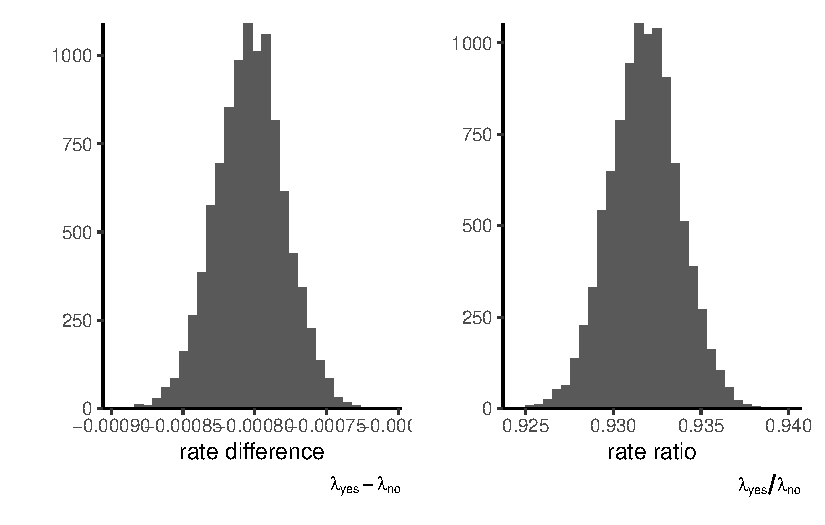
\includegraphics{priors_files/figure-pdf/fig-hist-difference_rates-1.pdf}

}

\caption{\label{fig-hist-difference_rates}Histograms of posterior
summaries for differences (left) and rates (right) based on 1000
simulations from the independent gamma posteriors.}

\end{figure}

To get an approximation to the posterior mean of the ratio
\(\lambda_1/\lambda_2\), it suffices to draw independent observations
from their respective posterior, compute the ratio and take the sample
mean of those draws. We can see that the sampling distribution of the
ratio is nearly symmetrical, so we can expect Wald intervals to perform
well should one be interested in building confidence intervals. This is
however hardly surprising given the sample size at play.

\end{example}

\begin{example}[Conjugate prior for Gaussian mean with known
variance]\protect\hypertarget{exm-conjugatepriors-normal}{}\label{exm-conjugatepriors-normal}

Consider an \(n\) simple random sample of independent and identically
distributed Gaussian variables with mean \(\mu\) and standard deviation
\(\sigma\), denoted \(Y_i \sim \mathsf{No}(\mu, \sigma^2)\). We pick a
Gaussian prior for the location parameter,
\(\mu \sim \mathsf{No}(\nu, \tau^2)\) where we assume \(\mu, \tau\) are
fixed hyperparameter values. For now, we consider only inference for
\(p(\mu \mid \sigma)\): discarding any term that is not a function of
\(\mu\), the conditional posterior is \begin{align*}
p(\mu \mid \sigma) &\propto \exp\left\{ -\frac{1}{2\sigma^2}\sum_{i=1}^n (y_{i}-\mu)^2\right\} \exp\left\{-\frac{1}{2\tau^2}(\mu - \nu)^2\right\}
\\&\propto p(\sigma)\sigma^{-1} \exp\left\{\left(\frac{\sum_{i=1}^n y_{i}}{\sigma^2} + \frac{\nu}{\tau^2}\right)\mu - \left( \frac{n}{2\sigma^2} +\frac{1}{2\tau^2}\right)\mu^2\right\}.
\end{align*} The log of the posterior density conditional on \(\sigma\)
is quadratic in \(\mu\), it must be a Gaussian distribution truncated
over the positive half line. This can be seen by completing the square
in \(\mu\), or by comparing this expression to the density of
\(\mathsf{No}(\mu, \sigma^2)\), \begin{align*}
f(x; \mu, \sigma) \stackrel{\mu}{\propto} \exp\left(-\frac{1}{2 \sigma^2}\mu^2 + \frac{x}{\sigma^2}\mu\right)
\end{align*} we can deduce by matching mean and variance that the
conditional posterior \(p(\mu \mid \sigma)\) is Gaussian with reciprocal
variance (precision) \(n/\sigma^2 + 1/\tau^2\) and mean
\((n\overline{y}\tau^2 + \nu \sigma^2)/(n\tau^2 + \sigma^2)\). The
precision is an average of that of the prior and data, but assigns more
weight to the latter, which increases linearly with the sample size
\(n\). Likewise, the posterior mean is a weighted average of prior and
sample mean, with weights proportional to the relative precision.

\end{example}

The exponential family is quite large;
\href{https://doi.org/10.1.1.157.5540}{Fink (1997) \emph{A Compendium of
Conjugate Priors}} gives multiple examples of conjugate priors and work
out parameter values.

In general, unless the sample size is small and we want to add expert
opinion, we may wish to pick an \emph{uninformative prior}, i.e., one
that does not impact much the outcome. For conjugate models, one can
often show that the relative weight of prior parameters (relative to the
random sample likelihood contribution) becomes negligible by
\href{https://en.wikipedia.org/wiki/Conjugate_prior}{investigating their
relative weights}.

\hypertarget{uninformative-priors}{%
\section{Uninformative priors}\label{uninformative-priors}}

\begin{definition}[Proper
prior]\protect\hypertarget{def-properprior}{}\label{def-properprior}

We call a prior function \emph{proper} if it's integral is finite over
the parameter space; such prior function automatically leads to a valid
posterior.

\end{definition}

The best example of prior priors arise from probability density
function. We can still employ this rule for improper priors: for
example, taking \(\alpha, \beta \to 0\) in the beta prior leads to a
prior proportional to \(x^{-1}(1-x)^{-1}\), the integral of which
diverges on the unit interval \([0,1]\). However, as long as the number
of success and the number of failures is larger than 1, meaning
\(k \geq 1, n-k \geq 1\), the posterior distribution would be proper,
i.e., integrable. To find the posterior, normalizing constants are also
superfluous.

Many uninformative priors are flat, or proportional to a uniform on some
subset of the real line and therefore improper. It may be superficially
tempting to set a uniform prior on a large range to ensure posterior
property, but the major problem is that a flat prior may be informative
in a different parametrization, as the following example suggests.

\begin{example}[Transformation of flat prior for
scales]\protect\hypertarget{exm-scaleflatprior}{}\label{exm-scaleflatprior}

Consider the parameter \(\log(\tau) \in \mathbb{R}\) and the prior
\(p( \log \tau) \propto 1\). If we reparametrize the model in terms of
\(\tau\), the new prior (including the Jacobian of the transformation)
is \(\tau^{-1}\)

\end{example}

Some priors are standard and widely used. In location scale families
with location \(\nu\) and scale \(\tau\), the density is such that
\begin{align*}
f(x; \nu, \tau) =  \frac{1}{\tau} f\left(\frac{x - \nu}{\tau}\right), \qquad \nu \in \mathbb{R}, \tau >0.
\end{align*} We thus wish to have a prior so that
\(p(\tau) = c^{-1}p(\tau/c)\) for any scaling \(c>0\), whence it follows
that \(p(\tau) \propto \tau^{-1}\), which is uniform on the log scale.

The priors \(p(\nu) \propto 1\) and \(p(\tau) \propto \tau^{-1}\) are
both improper but lead to location and scale invariance, hence that the
result is the same regardless of the units of measurement.

One criticism of the Bayesian approach is the arbitrariness of prior
functions. However, the role of the prior is often negligible in large
samples (consider for example the posterior of exponential families with
conjugate priors). Moreover, the likelihood is also chosen for
convenience, and arguably has a bigger influence on the conclusion. Data
fitted using a linear regression model seldom follow Gaussian
distributions conditionally, in the same way that the linearity is a
convenience (and first order approximation).

\begin{definition}[Jeffrey's
prior]\protect\hypertarget{def-jeffreys}{}\label{def-jeffreys}

In single parameter models, taking a prior function for \(\theta\)
proportional to the square root of the determinant of the information
matrix, \(p(\theta) \propto |\imath(\theta)|^{1/2}\) yields a prior that
is invariant to reparametrization, so that inferences conducted in
different parametrizations are equivalent.\footnote{The Fisher
  information is linear in the sample size for independent and
  identically distributed data so we can derive the result for \(n=1\)
  without loss of generality.}

To see this, consider a bijective transformation
\(\theta \mapsto \vartheta\). Under the reparametrized model and
suitable regularity conditions\footnote{Using Bartlett's identity;
  Fisher consistency can be established using the dominated convergence
  theorem.}, the chain rule implies that \begin{align*}
i(\vartheta) &= - \mathsf{E} \left(\frac{\partial^2 \ell(\vartheta)}{\partial^2 \vartheta}\right)
\\&= - \mathsf{E}\left(\frac{\partial^2 \ell(\theta)}{\partial \theta^2}\right) \left( \frac{\mathrm{d} \theta}{\mathrm{d} \vartheta} \right)^2 + \mathsf{E}\left(\frac{\partial \ell(\theta)}{\partial \theta}\right) \frac{\mathrm{d}^2 \theta}{\mathrm{d} \vartheta^2}
\end{align*} Since the score has mean zero,
\(\mathsf{E}\left\{\partial \ell(\theta)/\partial \theta\right\}=0\) and
the rightmost term vanishes. We can thus relate the Fisher information
in both parametrizations, with \begin{align*}
\imath^{1/2}(\vartheta) = \imath^{1/2}(\theta) \left| \frac{\mathrm{d} \theta}{\mathrm{d} \vartheta} \right|,
\end{align*} implying invariance.

Most of the times, Jeffrey's prior is improper. For the binomial model,
it can be viewed as a limiting conjugate beta prior with
\(\alpha, \beta\to 0\)). Unfortunately, in multiparameter models, the
system isn't invariant to reparametrization if we consider the
determinant of the Fisher information.

\end{definition}

\begin{example}[Jeffrey's prior for the binomial
distribution]\protect\hypertarget{exm-jeffreysbinom}{}\label{exm-jeffreysbinom}

Consider the binomial distribution
\(f(y; \theta, n) \propto \theta^y(1-\theta)^{n-y}\mathsf{I}_{\theta \in [0,1]}\).
The negative of the second derivative of the log likelihood with respect
to \(p\) is
\[\jmath(\theta) = - \partial^2 \ell(\theta; y) / \partial \theta^2 = y/\theta^2 + (1-y)/(1-\theta)^2\]
and since \(\mathsf{E}(Y)=n\theta\), the Fisher information is
\[\imath(\vartheta) = \mathsf{E}\{\jmath(\theta)\}=n/\theta + n/(1-\theta) = n/\{\theta(1-\theta)\}\]
Jeffrey's prior is thus
\(p(\theta) \propto \theta^{-1}(1-\theta)^{-1}\).

\end{example}

\hypertarget{exer-jeffreysnormal}{}
\hypertarget{jeffreys-prior-for-the-normal-distribution}{%
\section{Jeffrey's prior for the normal
distribution}\label{jeffreys-prior-for-the-normal-distribution}}

Check that for the Gaussian distribution \(\mathsf{No}(\mu, \sigma^2)\),
the Jeffrey's prior obtained by treating each parameter as fixed in
turn, are \(p(\mu) \propto 1\) and \(p(\sigma) \propto 1/\sigma\), which
also correspond to the default uninformative priors for location-scale
families.

\begin{example}[Jeffrey's prior for the Poisson
distribution]\protect\hypertarget{exm-jeffreyspoisson}{}\label{exm-jeffreyspoisson}

The Poisson distribution with
\(\ell(\lambda) \propto -\lambda + y\log \lambda\), with second
derivative
\(-\partial^2 \ell(\lambda)/\partial \lambda^2 = y/\lambda^2\). Since
the mean of the Poisson distribution is \(\lambda\), the Fisher
information is \(\imath(\lambda) = \lambda^{-1}\) and Jeffrey's prior is
\(\lambda^{-1/2}\).

\end{example}

\hypertarget{prior-simulation}{%
\section{Prior simulation}\label{prior-simulation}}

Oftentimes, expert elicitation is difficult and it is hard to grasp what
the impacts of the hyperparameters are. One way to see if the priors are
reasonable is to sample values from them and generate new observations,
resulting in prior predictive draws.

The prior predictive is
\(\int_{\boldsymbol{\Theta}} p(y \mid \boldsymbol{\theta}) p(\boldsymbol{\theta}) \mathrm{d} \boldsymbol{\theta}\):
we can simulate outcomes from it by first drawing parameter values from
the prior, then sampling new observations from the distribution in the
likelihood and keeping only the latter.

\begin{example}[]\protect\hypertarget{exm-bixi-temp}{}\label{exm-bixi-temp}

Consider the daily number of Bixi bike sharing users for 2017--2019 at
the Edouard Montpetit station next to HEC: we can consider a simple
linear regression with log counts as a function of
temperature,\footnote{If counts are Poisson, then the log transform is
  variance stabilizing.}
\[\log (\texttt{nusers}) \sim \mathsf{No}_{+}\{\beta_0 + \beta_1 (\texttt{temp}-20), \sigma^2\}.\]
The \(\beta_1\) slope measures units in degree Celsius per log number of
person.

The hyperparameters depend of course on the units of the analysis,
unless one standardizes response variable and explanatories: it is
easier to standardize the temperature so that we consider deviations
from, say 20\(^{\circ}\)C, which is not far from the observed mean in
the sample. After some tuning, the independent priors
\(\beta_0 \sim \mathsf{No}(\overline{y}, 0.5^2)\),
\(\beta_1 \sim \mathsf{No}(0, 0.05^2)\) and
\(\sigma \sim \mathsf{Exp}(3)\) seem to yield plausible outcomes and
relationships.\footnote{One can object to the prior parameters depending
  on the data, but an alternative would be to model centered data
  \(y-\overline{y}\), in which case the prior for the intercept
  parameter \(\beta_0\) would be zero.}

\begin{figure}[ht!]

{\centering 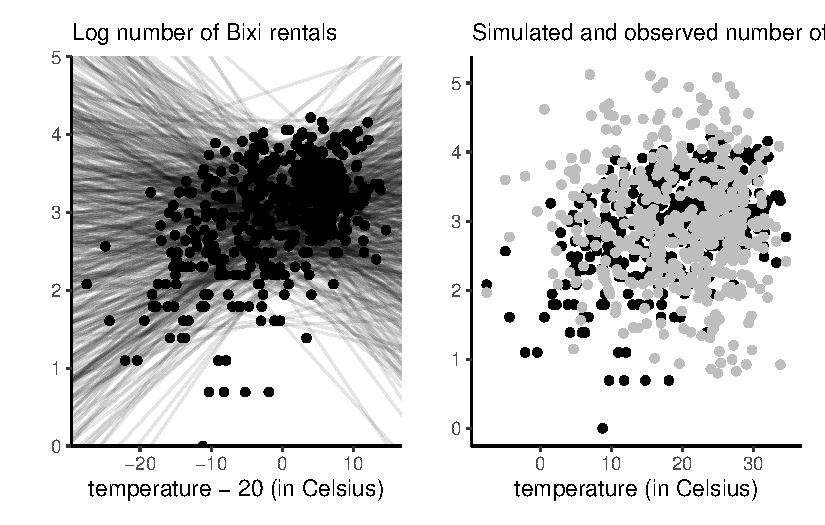
\includegraphics{priors_files/figure-pdf/fig-bixi-1.pdf}

}

\caption{\label{fig-bixi}Prior draws of the linear regressions with
observed data superimposed (left), and draws of observations from the
prior predictive distribution (in gray) against observed data (right).}

\end{figure}

We can draw regression lines from the prior, as in the left panel of
Figure~\ref{fig-bixi}: while some of the negative relationships appear
unlikely after seeing the data, the curves all seem to pass somewhere in
the cloud of point. By contrast, a silly prior is one that would result
in all observations being above or below the regression line, or yield
values that are much too large near the endpoints of the explanatory
variable. Indeed, given the number of bikes for rental is limited (a
docking station has only 20 bikes), it is also sensible to ensure that
simulations do not return overly large numbers. The maximum number of
daily users in the sample is 68, so priors that return simulations with
more than 200 (rougly 5.3 on the log scale) are not that plausible. The
prior predictive draws can help establish this and the right panel of
Figure~\ref{fig-bixi} shows that, expect for the lack of correlation
between temperature and number of users, the simulated values from the
prior predictive are plausible even if overdispersed.

\end{example}

\hypertarget{informative-priors}{%
\section{Informative priors}\label{informative-priors}}

One strength of the Bayesian approach is the capability of incorporating
expert and domain-based knowledge through priors. Often, these will take
the form of moment constraints, so one common way to derive a prior is
to perform moment matching to related ellicited quantities with moments
of the prior distribution. It may be easier to set priors on a different
scale than those of the observations, as Example~\ref{exm-colestawn}
demonstrates.

\begin{example}[Gamma quantile difference priors for extreme value
distributions]\protect\hypertarget{exm-colestawn}{}\label{exm-colestawn}

The generalized extreme value distribution arises as the limiting
distribution for the maximum of \(m\) independent observations from some
common distribution \(F\). The \(\mathsf{GEV}(\mu, \sigma, \xi)\)
distribution is a location-scale with distribution function
\begin{align*}
F(x) = \exp\left[ - \left\{1+\xi(x-\mu)/\sigma\right\}^{-1/\xi}_{+}\right]
\end{align*} where \(x_{+} = \max\{0, x\}\).

Inverting the distribution function yields the quantile function
\begin{align*}
Q(p) \mu + \sigma \frac{(-\log p)^{-\xi}-1}{\xi}
\end{align*}

In environmental data, we often model annual maximum. Engineering
designs are often specified in terms of the \(k\)-year return levels,
defined as the quantile of the annual maximum exceeded with probability
\(1/k\) in any given year. Using a \(\mathsf{GEV}\) for annual maximum,
Coles and Tawn (\protect\hyperlink{ref-Coles.Tawn:1996}{1996}) proposed
modelling annual daily rainfall and specifying a prior on the quantile
scale \(q_1 < q_2 < q_3\) for tail probabilities \(p_1> p_2 > p_3\). To
deal with the ordering constraints, gamma priors are imposed on the
differences \(q_1 - o \sim \mathsf{Ga}(\alpha_1, \beta_1)\),
\(q_2 - q_1 \sim \mathsf{Ga}(\alpha_2, \beta_2)\) and
\(q_3-q_2 \sim \mathsf{Ga}(\alpha_3, \beta_3)\), where \(o\) is the
lower bound of the support. The prior is thus of the form

\begin{align*}
p(\boldsymbol{q}) \propto q_1^{\alpha_1-1}\exp(-\beta_1 q_1) \prod_{i=2}^3 (q_i-q_{i-1})^{\alpha_i-1} \exp\{\beta_i(q_i-q_{i-1})\}.
\end{align*} where \(0 \leq q_1 \leq q_2 \leq q_3\). The fact that these
quantities refer to moments or risk estimates which practitioners often
must compute as part of regulatory requirements makes it easier to
specify sensible values for hyperparameters.

As illustrating example, consider maximum daily cumulated rainfall in
Abisko, Sweden. The time series spans from 1913 until December 2014; we
compute the 102 yearly maximum, which range from 11mm to 62mm, and fit a
generalized extreme value distribution to these.

For the priors, suppose an expert elicits quantiles of the 10, 50 and
100 years return levels; say 30mm, 45mm and 70mm, respectively, for the
median and likewise 40mm, 70mm and 120mm for the 90\% percentile of the
return levels. We can compute the differences and calculate the
parameters of the gamma distribution through moment-matching: this gives
roughly a shape of \(\alpha_1=18.27\) and \(\beta_1=0.6\), etc.
Figure~\ref{fig-gev-colestawn-quant-prior} shows the transfer from the
prior predictive to the posterior distribution. The prior is much more
dispersed and concentrated on the tail, which translates in a less
peaked posterior than using a weakly informative prior (dotted line):
the mode of the latter is slightly to the left and with lower density in
the tail.

\begin{figure}[ht!]

{\centering 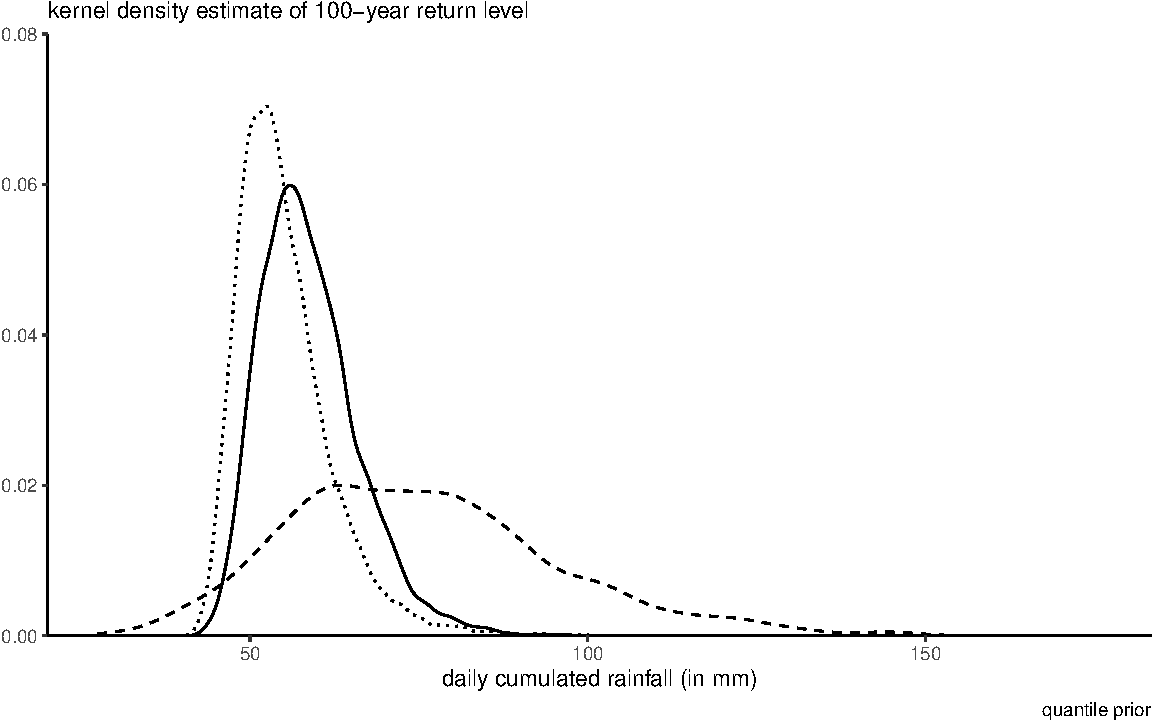
\includegraphics{priors_files/figure-pdf/fig-gev-colestawn-quant-prior-1.pdf}

}

\caption{\label{fig-gev-colestawn-quant-prior}Kernel density estimates
of draws from the posterior distribution of 100 year return levels with
a Coles--Tawn quantile prior (full line) and from the corresponding
prior predictive (dashed). The dotted line gives the posterior
distribution for a maximum domain information prior on the shape with
improper priors on location and scale.}

\end{figure}

\end{example}

What would you do if we you had prior information from different
sources? One way to combine these is through a mixture: given \(M\)
different prior distributions \(p_m(\boldsymbol{\theta})\), we can
assign each a positive weight \(w_m\) to form a mixture of experts prior
through the linear combination
\[ p(\boldsymbol{\theta}) \propto \sum_{m=1}^M w_m p_m(\boldsymbol{\theta})\]

\hypertarget{priors-for-regression-models}{%
\section{Priors for regression
models}\label{priors-for-regression-models}}

Gaussian components are widespread: not only for linear regression
models, but more generally for the specification of random effects that
capture group-specific effects, residuals spatial or temporal
variability. In the Bayesian paradigm, there is no difference between
fixed effects \(\boldsymbol{\beta}\) and the random effect parameters:
both are random quantities that get assigned priors.

It is generally good advice to center and scale explanatory variables
and response vectors so they have approximately mean zero and unit
variance, as this facilitates prior specification.

Andrew Gelman uses the following taxonomy for various levels of prior
information: uninformative priors are generally flat or uniform priors
with \(p(\beta) \propto 1\), vague priors are typically nearly flat even
if propor, e.g., \(\beta \sim \mathsf{No}(0, 100)\), weakly informative
priors provide little constraints \(\beta \sim \mathsf{No}(0, 10)\)),
and informative prior are typically application-specific, but constrain
the ranges. Uninformative and vague priors are not recommended.

If Gaussian priors are ubiquitous for the mean parameters
\(\boldsymbol{\beta}\), priors for the scale are more contentious.
Gelman (\protect\hyperlink{ref-Gelman:2006}{2006}) recommends a
Student-\(t\) distribution truncated below at \(0\), with low degrees of
freedom.

The rationale for this choice comes from the simple two level model:
\begin{align*}
Y_{ij} &\sim \mathsf{No}(\mu + \alpha_j, \sigma^2), \qquad i=1,\ldots, n_j; j = 1, \ldots, J \\
\alpha_j &\sim \mathsf{No}(0, \tau^2_\alpha), \qquad j =1, \ldots, J
\end{align*} Given \(\alpha, \mu, \sigma\) and the data
\(\boldsymbol{y}\), the conditionally conjugate prior is inverse gamma.
Standard inference with this parametrization is complicated, because
there is strong dependence between parameters.

To reduce this dependence, one can consider an overparametrization in
which \(\alpha_j = \xi \eta_j\) and
\(\eta_j \sim \mathsf{No}(0, \tau^2_\eta)\), where now
\(\tau_\alpha=|\xi|\tau_{\eta}\) so there is an additional parameter.
Consider the likelihood conditional on \(\mu, \eta_j\): we have that
\((y_{ij} - \mu)/\eta_j \sim \mathsf{No}(\xi, \sigma^2/\eta_j)\) so
conditionally conjugate priors for \(\xi\) and \(\tau_\eta\) are
respectively Gaussian an inverse-gamma. This translates into a prior
distribution for \(\tau_\alpha\) which is that of the absolute value of
a noncentral Student-\(t\) with location, scale and degrees of freedom
\(\nu\). If we set the location to zero, the prior puts high mass at the
origin, but is heavy tailed with polynomial decay. We recommend to set
degrees of freedom so that the variance is heavy-tailed, e.g.,
\(\nu=3\). While this prior is not conjugate, it compares favorably to
the \(\mathsf{IGa}(\epsilon, \epsilon)\) that used to be widespread with
\(\epsilon>0\) typically set to \(0.01\) or \(0.001\), approaching an
improper prior. Posterior inference is unfortunately sensitive to the
value of \(\epsilon\) in hierarchical models when the random effect
variance is close to zero, and more so when there are few levels for the
groups since the relative weight of the prior relative to that of the
likelihood contribution is then large.

\begin{example}[Poisson random effect
models]\protect\hypertarget{exm-randomeffects}{}\label{exm-randomeffects}

We consider data from an experimental study conducted at Tech3Lab on
road safety. In Brodeur et al.
(\protect\hyperlink{ref-Brodeur:2021}{2021}), 31 participants were asked
to drive in a virtual environment; the number of road violation was
measured for different type of distractions (phone notification, phone
on speaker, texting and smartwatch). The data are balanced, with each
participant exposed to each task exactly once.

We model the data using a Poisson mixed model to measure the number of
violations, \texttt{nviolation}, with a fixed effect for \texttt{task},
which captures the type of distraction, and a random effect for
participant \texttt{id}. The hierarchical model fitted for individual
\(i\) and distraction type \(j\) is \begin{align*}
Y_{ij} &\sim \mathsf{Po}\{\mu = \exp(\beta_{j} + \alpha_i)\}, \qquad i = 1, \ldots, 31; j = 1, \ldots, 4\\
\beta_j &\sim \mathsf{No}(0, 100) \qquad   j = 1, \ldots, 4\\
\alpha_i &\sim \mathsf{No}(0, \kappa^2); \qquad i=1, \ldots, 31
\kappa \sim \mathsf{St}_{+}(3)
\end{align*} so observations are conditionally independent given
hyperparameters \(\alpha\) and \(\beta\).

In frequentist statistics, there is a distinction made in mixed-effect
models between parameters that are treated as constants, termed fixed
effects and corresponding in this example to \(\boldsymbol{\beta}\), and
random effects, equivalent to \(\boldsymbol{\alpha}\). There is no such
distinction in the Bayesian paradigm, except perhaps for the choice of
prior.

We can look at some of posterior distribution of the 31 random effects
(here the first five individuals) and the fixed effect parameters
\(\boldsymbol{\beta}\), plus the variance of the random effect
\(\kappa\): there is strong evidence that the latter is non-zero,
suggesting strong heterogeneity between individuals. The distraction
which results in the largest number of violation is texting, while the
other conditions all seem equally distracting on average (note that
there is no control group with no distraction to compare with, so it is
hard to draw conclusions).

\begin{figure}[ht!]

{\centering 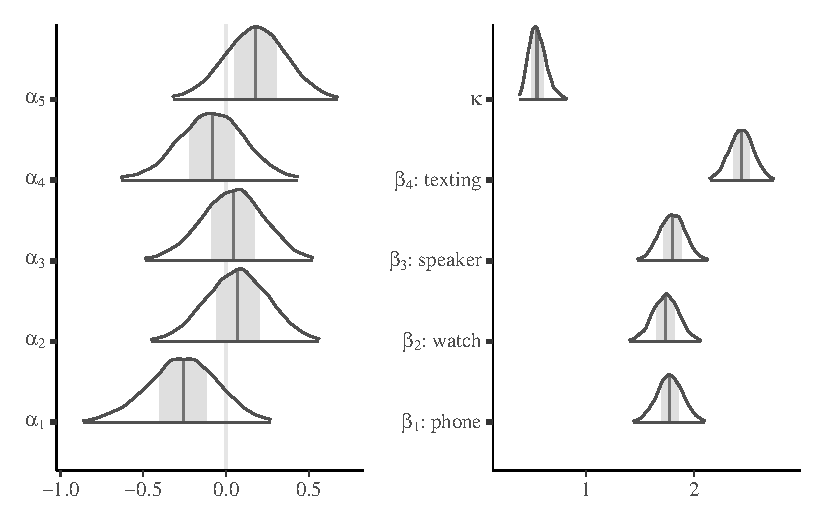
\includegraphics{priors_files/figure-pdf/fig-post-dist-poisson-mixed-1.pdf}

}

\caption{\label{fig-post-dist-poisson-mixed}Posterior density plots with
50\% credible intervals and median value for the random effects of the
first five individuals (left) and the fixed effects and random effect
variance (right).}

\end{figure}

\end{example}

\hypertarget{penalized-complexity-priors}{%
\section{Penalized complexity
priors}\label{penalized-complexity-priors}}

Oftentimes, there will be a natural family of prior density to impose on
some model component, \(p(\boldsymbol{\theta} \mid \zeta)\), with
hyperparameter \(\zeta\). The flexibility of the underlying construction
leads itself to overfitting. Penalized complexity priors
(\protect\hyperlink{ref-Simpson:2017}{Simpson et al. 2017}) aim to
palliate this by penalizing models far away from a simple baseline
model, which correspond to a fixed value \(\zeta_0\). The prior will
favour the simpler parsimonious model the more prior mass one places on
\(\zeta_0\), which is in line with Occam's razor principle.

To construct a penalized-complexity prior, we compute the
Kullback--Leibler divergence between the model
\(p_\zeta \equiv p(\boldsymbol{\theta} \mid \zeta)\) relative to the
baseline with \(\zeta_0\),
\(p_0 \equiv p(\boldsymbol{\theta} \mid \zeta_0)\); the
Kullback--Leibler divergence is

\[
\mathsf{KL}(p_\zeta \Vert\, p_0)=\int p_\zeta \log\left(\frac{p_\zeta}{p_0}\right) \mathrm{d} \boldsymbol{\theta}.
\] The distance between the prior densities is then set to
\(d(\zeta) = \{2\mathsf{KL}(p_\zeta \mid\mid p_0)\}^{1/2}\). which is
zero at the model with \(\zeta_0\). The PC prior then constructs an
exponential prior on the distance scale, which after back-transformation
gives
\(p(\zeta \mid \lambda) = \lambda\exp(-\lambda d(\zeta)) \left| {\partial d(\zeta)}/{\partial \zeta}\right|\).
To choose \(\lambda\), the authors recommend elicitation of a pair
\((U, \alpha)\) such that \(\Pr(\lambda > U)=\alpha\).

\begin{example}[Penalized complexity prior for random effects
models]\protect\hypertarget{exm-pcprior-randomeffect}{}\label{exm-pcprior-randomeffect}

Simpson et al. (\protect\hyperlink{ref-Simpson:2017}{2017}) give the
example of a Gaussian prior for random effects \(\boldsymbol{\alpha}\),
of the form
\(\boldsymbol{\alpha} \mid \zeta \sim \mathsf{No}_J(\boldsymbol{0}_J, \zeta^2 \mathbf{I}_J)\)
where \(\zeta_0=0\) corresponds to the absence of random
subject-variability. The penalized complexity prior for the scale
\(\zeta\) is then an exponential with rate \(\lambda\),\footnote{Possibly
  truncated above if the support of \(\zeta\) has a finite upper bound.}
with density \(p(\zeta \mid \lambda) = \lambda \exp(-\lambda \zeta)\).
Using the recommendation for setting \(\lambda\), we get that
\(\lambda = -\ln(\alpha/U)\) and this can be directly interpreted in
terms of standard deviation of \(\zeta\); simulation from the prior
predictive may also be used for calibration.

\end{example}

\begin{example}[Penalized complexity prior for autoregressive model of
order
1]\protect\hypertarget{exm-pcprior-arorder}{}\label{exm-pcprior-arorder}

Sørbye and Rue (\protect\hyperlink{ref-Sorbye.Holbek.Rue:2017}{2017})
derive penalized complexity prior for the Gaussian stationary AR(1)
model with autoregressive parameter \(\phi \in (-1,1)\), where
\(Y_t \mid Y_{t-1}, \phi, \sigma^2 \sim \mathsf{No}(\phi Y_{t-1}, \sigma^2)\).
There are two based models that could be of interest: one with
\(\phi=0\), corresponding to lack of autocorrelation, and a static mean
\(\phi=1\) for no change in time, which is not stationary. For the
former, the penalized complexity prior is \begin{align*}
p(\phi \mid \lambda) = \frac{\lambda}{2} \exp\left[-\lambda \left\{-\ln(1-\phi^2)\right\}^{1/2}\right] \frac{|\phi|}{(1-\phi^2)\left\{-\ln(1-\phi^2)\right\}^{1/2}}.
\end{align*} One can set \(\lambda\) by considering plausible values by
relating the parameter to the variance of the one-step ahead forecast
error.

\end{example}

\hypertarget{sensitivity-analysis}{%
\section{Sensitivity analysis}\label{sensitivity-analysis}}

Do priors matter? The answer to that question depends strongly on the
model, and how much information the data provides about hyperparameters.
While this question is easily answered in conjugate models (the relative
weight of hyperparameters relative to data can be derived from the
posterior parameters), it is not so simple in hierarchical models, where
the interplay between prior distributions is often more intricate. To
see the impact, one often has to rely on doing several analyses with
different values fr the prior and see the sensitivity of the conclusions
to these changes, for example by considering a vague prior or modifying
the parameters values (say halving or doubling). If the changes are
immaterial, then this provides reassurance that our analyses are robust.

\begin{example}[]\protect\hypertarget{exm-sensitivity-poisson-mixed}{}\label{exm-sensitivity-poisson-mixed}

To check the sensitivity of the conclusion, we revisit the modelling of
the \texttt{smartwatch} experiment data using a Poisson regression and
compare four priors: a uniform prior truncated to \([0, 10]\), an
inverse gamma \(\mathsf{IG}(0.01, 0.01)\) prior, a penalized complexity
prior such that the 0.95 percentile of the scale is 5, corresponding to
\(\mathsf{Exp}(0.6)\). Since each distraction type appears 31 times,
there is plenty of information to reliably estimate the dispersion
\(\kappa\) of the random effects \(\alpha\): the different density plots
in Figure~\ref{fig-sensitivity} are virtually indistinguishable from one
another.

\begin{figure}[ht!]

{\centering 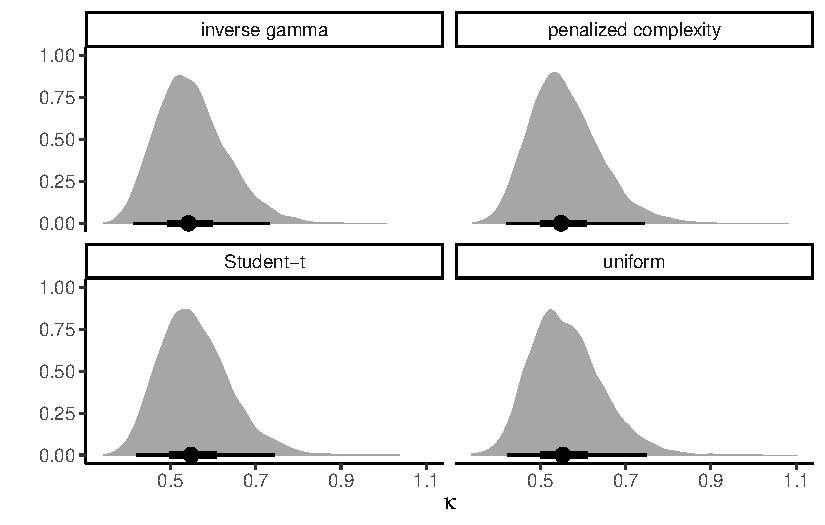
\includegraphics{priors_files/figure-pdf/fig-sensitivity-1.pdf}

}

\caption{\label{fig-sensitivity}Posterior density of the scale of the
random effects with uniform, inverse gamma, penalized complexity and
folded Student-t with three degrees of freedom. The circle denotes the
median and the bars the 50\% and 95\% percentile credible intervals.}

\end{figure}

\end{example}

\bookmarksetup{startatroot}

\hypertarget{references}{%
\chapter*{References}\label{references}}
\addcontentsline{toc}{chapter}{References}

\markboth{References}{References}

\hypertarget{refs}{}
\begin{CSLReferences}{1}{0}
\leavevmode\vadjust pre{\hypertarget{ref-Alexander:2023}{}}%
Alexander, Rohan. 2023. \emph{Telling Stories with Data: With
Applications in {R}}. Boca Raton, FL: CRC Press.

\leavevmode\vadjust pre{\hypertarget{ref-Brodeur:2021}{}}%
Brodeur, Mathieu, Perrine Ruer, Pierre-Majorique Léger, and Sylvain
Sénécal. 2021. {``Smartwatches Are More Distracting Than Mobile Phones
While Driving: Results from an Experimental Study.''} \emph{Accident
Analysis \& Prevention} 149: 105846.
\url{https://doi.org/10.1016/j.aap.2020.105846}.

\leavevmode\vadjust pre{\hypertarget{ref-Coles.Tawn:1996}{}}%
Coles, Stuart G., and Jonathan A. Tawn. 1996. {``A {B}ayesian Analysis
of Extreme Rainfall Data.''} \emph{Journal of the Royal Statistical
Society. Series C (Applied Statistics)} 45 (4): 463--78.
\url{https://doi.org/10.2307/2986068}.

\leavevmode\vadjust pre{\hypertarget{ref-deFinetti:1974}{}}%
Finetti, Bruno de. 1974. \emph{Theory of Probability: A Critical
Introductory Treatment}. Vol. 1. New York: Wiley.

\leavevmode\vadjust pre{\hypertarget{ref-Gelfand.Smith:1990}{}}%
Gelfand, Alan E., and Adrian F. M. Smith. 1990. {``Sampling-Based
Approaches to Calculating Marginal Densities.''} \emph{Journal of the
American Statistical Association} 85 (410): 398--409.
\url{https://doi.org/10.1080/01621459.1990.10476213}.

\leavevmode\vadjust pre{\hypertarget{ref-Gelman:2006}{}}%
Gelman, Andrew. 2006. {``Prior Distributions for Variance Parameters in
Hierarchical Models (Comment on Article by {B}rowne and {D}raper).''}
\emph{Bayesian Analysis} 1 (3): 515--34.
\url{https://doi.org/10.1214/06-BA117A}.

\leavevmode\vadjust pre{\hypertarget{ref-Geman.Geman:1984}{}}%
Geman, Stuart, and Donald Geman. 1984. {``Stochastic Relaxation, {G}ibbs
Distributions, and the {B}ayesian Restoration of Images.''} \emph{IEEE
Transactions on Pattern Analysis and Machine Intelligence} PAMI-6 (6):
721--41. \url{https://doi.org/10.1109/TPAMI.1984.4767596}.

\leavevmode\vadjust pre{\hypertarget{ref-Matias:2021}{}}%
Matias, J. Nathan, Kevin Munger, Marianne Aubin Le Quere, and Charles
Ebersole. 2021. {``The {U}pworthy {R}esearch {A}rchive, a Time Series of
32,487 Experiments in {U.S.} Media.''} \emph{Scientific Data} 8 (195).
\url{https://doi.org/10.1038/s41597-021-00934-7}.

\leavevmode\vadjust pre{\hypertarget{ref-McNeil.Frey.Embrechts:2005}{}}%
McNeil, A. J., R. Frey, and P. Embrechts. 2005. \emph{Quantitative Risk
Management: Concepts, Techniques, and Tools}. 1st ed. Princeton, NJ:
Princeton University Press.

\leavevmode\vadjust pre{\hypertarget{ref-Simpson:2017}{}}%
Simpson, Daniel, Håvard Rue, Andrea Riebler, Thiago G. Martins, and
Sigrunn H. Sørbye. 2017. {``Penalising Model Component Complexity: A
Principled, Practical Approach to Constructing Priors.''}
\emph{Statistical Science} 32 (1): 1--28.
\url{https://doi.org/10.1214/16-STS576}.

\leavevmode\vadjust pre{\hypertarget{ref-Sorbye.Holbek.Rue:2017}{}}%
Sørbye, Sigrunn Holbek, and Håvard Rue. 2017. {``Penalised Complexity
Priors for Stationary Autoregressive Processes.''} \emph{Journal of Time
Series Analysis} 38 (6): 923--35.
\url{https://doi.org/10.1111/jtsa.12242}.

\end{CSLReferences}


\backmatter

\end{document}
